\section{Introduction}

Evolutionary algorithms are classified as meta-heuristic search algorithms, where possible solution elements span the n-dimensional search space to find the global optimum solution. Over the years, natural phenomena and biological processes have laid the foundation for several algorithms for control and optimization that have highlighted their applicability in solving intricate optimization problems. For instance, at the cellular level in the E.Coli Bacterium, there is sensing and locomotion involved in seeking nourishment and avoiding harmful chemicals. These behavioral characteristics fuelled the inspiration for the Bacterial Foraging Optimization algorithm \cite{passino2002biomimicry}\cite{onwubolu2013new}. Ant Colony Optimization \cite{dorigo2010ant} deals with behavior of ants and has been a successful model for solving complex problems. Particle Swarm Optimization \cite{kennedy2011particle} is a swarm intelligence algorithm based on behavior of birds and fishes that models these particles as they traverse an n-dimensional search space and share information in order to obtain global optimum.
From a biological control point, the human brain represents one of the most advanced architectures and several research attempts seek to mimic its functional accuracy, precision and efficiency. The brain function activities can be broadly classified into 2 categories: sensory and motor operations. Sensory cortical functions inspired the concept of neural networks that are being scaled successfully in deep learning to solve vast amount of problems.

\begin{figure}[h!]
  \includegraphics[scale=0.6]{motorControl}
  \caption{Hierarchy of Motor Control in Humans}
  \label{fig:motorControl}
\end{figure}

The human motor function represents a distributed neural and hierarchical control system. It can be classified as having local control functions for movement as well as higher level controllers for gross motion and decision making. The execution of motor operation involves distributed brain structures at different levels of hierarchy. These include the pre-frontal cortex, motor cortex, spinal cord, anterior horn cells etc \cite{Shaw1982119}. For executing an action sequence, a sequence of actions is implemented by a string of subsequences of actions each implemented in a different part of the body. The operational structure has been depicted in Figure 1\cite{passino2005biomimicry}.
For optimality of actions, neurons act in unison. The neurons in the motor cortex act like global leaders and send inhibitory or facilitatory influence over anterior horn cells, the local leaders, located in the spinal cord\cite{Shaw1982119}. These local leaders are connected to muscle fibers, the effectors, through a peripheral nerve and neuromuscular junction.
Efficient execution of task requires feedback based facilitation and inhibition of the effectors over the anterior horn cells. These sequence of operations realise the optimal convergence of the system leading to smooth motor execution.


The present work introduces an algorithm modelled intuitively on the distributed and hierarchical operation of the brain motor function.     

The Classical DE Algorithm \cite{storn1995differential}, proposed by Storn and Price has been hailed as one of the premier evolutionary algorithms, owing to its simple yet effective structure\cite{das2011differential}. However, in recent times, it has been criticized for its slow convergence rate and inability to effectively optimize multimodal composite functions\cite{das2011differential}. This work focusses on supplementing the algorithm's performance through the introduction of hierarchical influence in the pipeline. The architecture enables the algorithm to control the flow of agents through the cummulative effect of global and local leaders in the hierarchy. \\
The proposed approach, Hierarchy Influenced Differential Evolution (HIDE), has been subjected to exhaustive analysis on the hybrid and composite objective functions of the CEC 2017 benchmark\cite{cec2017benchmark}. Comparison with the classical DE algorithm and its other popular variants including JADE and PSODE \cite{zhang2009jade} highlights the particular viability of the schemed approach in solving complex optimization tasks. We show that even with fixed parameters, HIDE is able to outperform adaptive architectures such as JADE by a respectable margin, as discussed in the result sections.



% Operational maturity of biological control systems have enamored researchers across various domains.Consequently, these have been the source of inspiration of various mathematical and logical models for control, automation and optimization. The behavioral characteristics observed at the Cellular level in E.Coli fueled the inspiration for the Bacterial Foraging Optimization algorithm.

% The biological system most relevant to us is the human brain. It represents the most advanced control architecture and several research initiative seek to mimic its level of accuracy and precision in day-to-day activities. The brain activities can be distributed into two categories: sensory and motor operations. Sensory cortical functions have to an extent inspired the concept of neural networks that have been successfully scaled to a large number of domains. 

% While not always the case, it is at times useful and accurate to view a biological neural network as being arranged in a hierarchical fashion. As a naive example, consider a day-to-day activity of grasping a cup of coffee.
% One part of the brain that is clearly hierarchical is the human motor system. The hierarchical and distributed control of the human motor system can be classified as having local control functions for movement and higher level controllers that facilitate gross motion and decision making.

% The optimal execution of any human motor operation, such as grasping a cup of coffee, involves distributed brain structures at different levels of hierarchy. It broadly includes the prefrontal cortex, motor cortex, spinal cord, anterior horn cells etc. In generating actions sequences, a sequence of actions is implemented by string of subsequences of actions, each possibly implemented in different parts of the body.

% The hierarchy of the operations can be classified as:

% \begin{itemize}
% \item[1.] Motivation and planning of the movement or task.
% \item[2.] Generation of instructions for movement.
% \item[3.] Refinement of instruction based on feedback from components.
% \item[4.] Maintenance of posture and smooth execution of task.
% \end{itemize}

% Whenever a person plans to perform an action, electrical signal generated from the pyramidal neurons in the prefrontal cortex(global leaders, center for the decision making) are transmitted a supraspinal tract on the anterior horn cells(communicating to local leaders). Initially, these global leaders send inhibitory influence to the population over the local leaders. Efficient and optimal execution of tasks involves feedback based facilitation and inhibition of the effectors. These result in contraction and relaxation of the agonist and antagonist muscle fibers through the local leaders. The sequence of updation of the represents the optimal convergence of the system, leading to smooth motor operations.

\section{Classical Differential Evolution}

The classical Differential Evolution (DE) algorithm is a population-based global optimization algorithm, utilizing a crossover and mutation approach to generate new individuals in the population for achieving optimum solutions\cite{das2011differential}. For each individual $x_i$ that belongs to the population for generation $G$, DE randomly samples three individuals from the population namely $x_{r1,G}$, $x_{r2,G}$ and $x_{r3,G}$. Employing these randomly chosen points, a new individual trial vector, $v_i$, is generated using equation \eqref{de}:

\begin{equation}
\label{de}
v_i = x_{r1,G} + F (x_{r2,G} - x_{r3,G})
\end{equation}

Where, $F$ is called the differential weight (Usually lies between $[0, 1]$).\\
To obtain the updated position of the individual, a crossover operation is implemented between $x_{i,G}$ and $v_i$, controlled by the parameter $CR$ called the crossover probability. The value for $CR$ always lies between $[0, 1]$.

\begin{figure}[h!]
  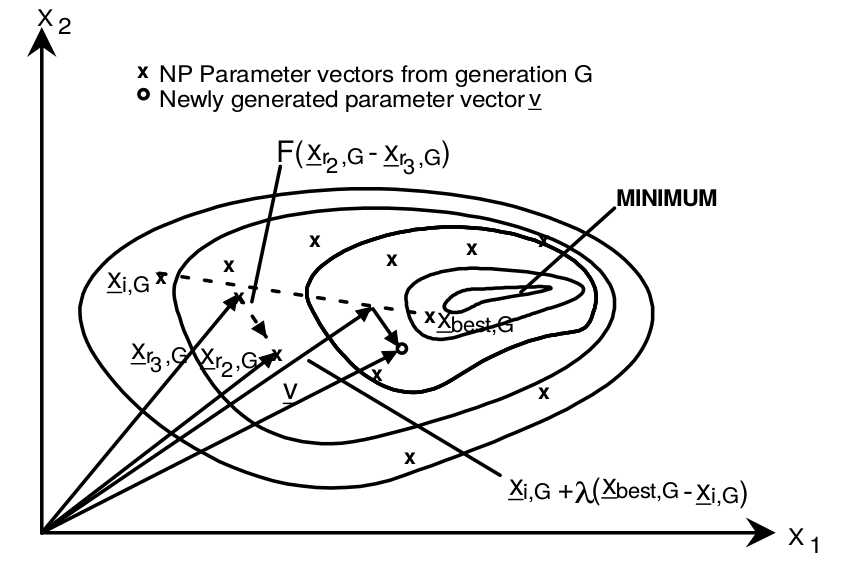
\includegraphics[scale=0.3]{contourDE}
 \caption{Motion planning of individuals in DE on two dimensional example of objective function.}

  \label{fig:contourDE}
\end{figure}

%%%%%%%%%%%%%%%%%%%%%%%%%%%%%%%%%%%%%%%%%%%%%%%%%%%%%%%%%%%%%%%%%%%%%%%%%%%%%%%%%%%%%%%%%%%%%%%%%%%%%%%%%%%%%%

\section{Hierarchy Influenced Differential Evolution}

Taking inspiration from the human motor system, we model the hierarchical motor operations in our optimization agents, where we define a global leader which influences the action of several distributed local leaders and the particle agents which act as the effectors. The global leader is analogous to the decision making and planning section in the motor system hierarchy whilst, the local leaders correspond to motion generators acting under the influence of the  global leader.


The position of each particle in the population is affected by the influence of global leader and local leaders, while also being affected by a randomly chosen particle from the population to induce some stochasticity in the optimization pipeline. We first model the influence of the global leader on the local leaders and the influences of the local leaders  on each population element using equation \eqref{one} and \eqref{two}. We introduce a hierarchical crossover between the two influencing equations governed by a hierarchical crossover parameter $HC$.


        % \For{each dimension $j$}
        %   \If {$random(0, 1) \textless HC$}
        %     \State Set $x'_{j,i} = x_{j,i,G}$.
        %   \Else
        %     \State Set $x'_{j,i} = u_{j,i}$
        %   \EndIf
        % \EndFor

\begin{algorithm}[b]
\caption{Hierarchy Influenced Differential Evolution}
\label{algo}
\begin{algorithmic}[1]
  \Procedure{Start}{}
    \State Initialize parameters ($HC$, $F$, $P$, $N_l$, $NP$).
    \State Generate initial global leader $g_L$ as a random point.
    \State Generate $N_l$ local leader points around $g_L$ global leader.
    \State Using a Normal distribution, generate $NP$ points for population $P$ around the local leaders.
    \While{termination criteria is not met}
    %%%%%%%%%%%%%%%%%%%%%%%%%%%%%%%%%%%%%%%%%%%%%%%%%%%%%%%%%%%%%%%%%%%%%%%%%%%%%%%%%%%%%%
      \For{each individual $x_{i,G}$ in $P$}
        \State Determine the corresponding local leader $x_{L_i,G}$ from the set of all local leader based on nearest position.
        \State Let $u = 0$ be an empty vector.
        \State Let $G$ and $G_{t}$ be the current generation and total generations of the procedure.
        \If {$G == (HC * G_{t})$}
          \State Increase the population : $G_{t} = 2 * G_{t}$
        \EndIf
        \If {$G < (HC * G_{t})$}
          \State $u_i = E_g$ from \eqref{one}.
        \Else
          \State $u_i = E_l$ from \eqref{two}.
        \EndIf
        \State $x'_{i}$ = BinomialCrossover($u_{i}$, $x_{i,G}$, $CR$)
        \If {$f(x'_{i})$ < $f(x_{i,G})$}
          \State Replace $x_{i,G}$ with $x'_{i}$ in the next generation.
        \EndIf
      \EndFor
      \State Alter local leaders in each population cluster based on objective function value.
      \State Compute updated global leader $g_L$.
    \EndWhile
  \EndProcedure
\end{algorithmic}
\end{algorithm}

\begin{algorithm}[b]
\caption{Binomial\_Crossover($u$, $x$, $CR$)}
\label{algo}
\begin{algorithmic}[1]
  \Procedure{Start}{}
    \State Let $x' = 0$ be an empty vector.
    \State Select a random integer k = $irand$(\{1,2,...,d\}); where d = number of dimensions
    \For{each dimension $j$}
      \If {$random(0, 1) \textless CR$ \textbf{or} $j==k$}
        \State Set $x'_{j} = u_{j}$
      \Else
        \State Set $x'_{j} = x_{j}$
      \EndIf
    \EndFor
  \EndProcedure
\end{algorithmic}
\end{algorithm}


Analogously to the brain motor operation as depicted in Figure 1, the update of particle positions requires generating feedback for the leaders as a part of the optimization procedure, and hence the local leaders and the global leader are updated based on their objective function value generated from the perturbations in population particles. This series of events comprise of one optimization pass (one generation step). On execution of several optimization passes as described, the system is able to converge to an optimal configuration, analogous to the successful execution of the required task as shown in the final steps of Figure 1.

For each particle $x_{i,G}$, $i = 0, 1, 2,...NP-1$ for generation G, the trial vector $x'_{i}$ of the particle, is governed by the hierarchical crossover operation and a mutation operation as follows : 

\vspace{-1.5mm}
\begin{equation}
u_i =  
\left\{
\begin{array}{ll}
      E_g, & if \thinspace\thinspace G < HC * G_{t} \\
      E_l, & otherwise \\
\end{array} 
\right. 
\end{equation}\\

\vspace{-5.5mm}
\begin{equation}
\label{one}
E_g = g_L + F (x_{L_i,G} - x_{r,G})
\end{equation}

\vspace{-1.5mm}
\begin{equation}
\label{two}
E_l = x_{L_i,G} + F (x_{i,G} - x_{r,G})
\end{equation}

for each dimension $j$ of $x_{j,i,G}$:
\begin{equation}
x'_{j,i} =  
\left\{
\begin{array}{ll}
      x_{j,i,G} & if \thinspace\thinspace rand(0,1) < HC \\
      u_{j,i} & otherwise \\
\end{array} 
\right. 
\end{equation}\\
\vspace{-5.5mm}

\vspace{-1.5mm}
\begin{equation}
x_{i,G+1} =  
\left\{
\begin{array}{ll}
      x'_{i,G}, & if \thinspace\thinspace f(x'_{i,G}) < f(x_{i,G}) \\
      x_{i,G}, & otherwise \\
\end{array} 
\right. 
\end{equation}\\
\vspace{-2mm}


\begin{figure}[h!]
  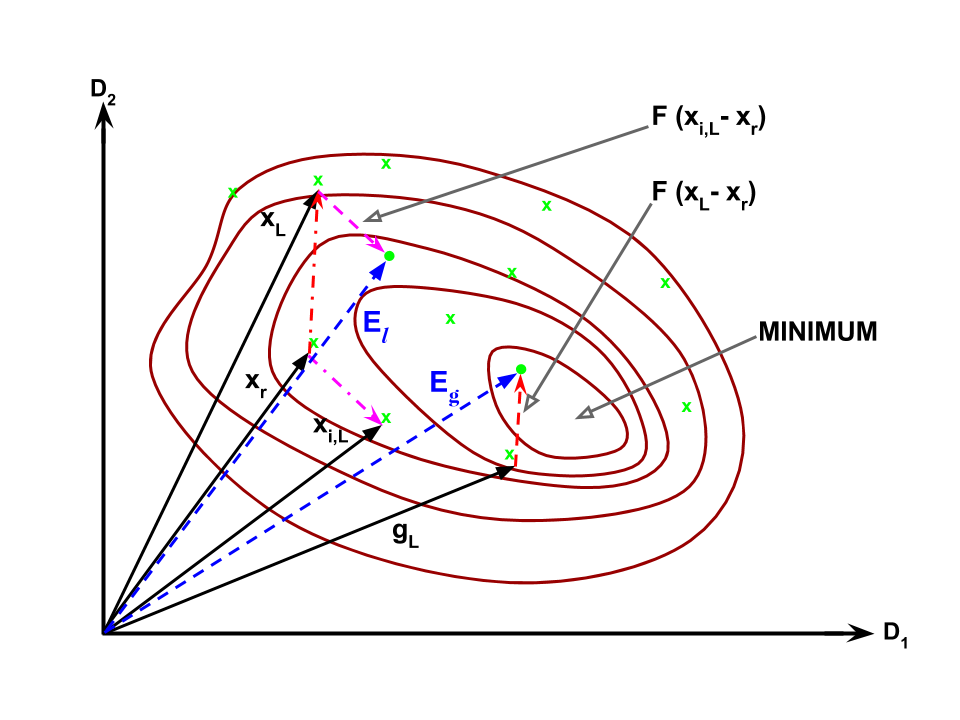
\includegraphics[scale=0.25]{contourDL}
  \caption{Hierarchical Decisive Motion planning of individuals in HIDE on two dimensional example of objective function. The position vectors resulting from the influence of global leader and local leaders are both represented
as E$_{g}$ and E$_{l}$ on the contour of a two dimensional objective function.}
  \label{fig:contourDL}
\end{figure}


where, \\
$G_{t}$ is the total number of generations,\\
$x_{i,G+1}$ is the vector position of $x_{i,G}$ for next generation\\
$F$ is factor responsible for amplification of differential variation, \\
$f$ is the objective function, \\
$x_{i,G}$ is the current position of the individual for generation G,\\
$u_i$ is the intermediate trial vector of the current individual,\\
$E_g$ represents the global and local leader interaction,\\
$E_l$ represents the local leader and effector interaction,\\
$g_L$ is the global leader for generation G, \\
$x_{L_i,G}$ is the position of the local leader for current individual,\\
$x_{r,G} \epsilon$ P $;$  \thinspace r $\epsilon$ [0,1,.. NP-1] \\
$x'_{j,i}$ is the trial vector\\

$x_{r,G}$ is randomly chosen particle from the population to induce stochasticity. The hierarchical operation is affected by the global leader $g_L$ and the local leader $x_{L_i,G}$  through the parametric equations \eqref{one} and \eqref{two}. Switching between the two is governed by the hierarchical crossover parameter $HC$.


\subsection{Hierarchical Crossover}

Convergence trend in HIDE is largely pivoted about (3) and (4), which in unison, lend a hierarchical structure to the algorithm. A successful optimization algorithm involves establishing a trade-off between exploration and exploitation. Achieving global optimization can be visualized as collaboration of two forces, exploration over a larger subspace followed by intensive exploitation over the resulting search space governed by clusters. Phase 1, involving (3) is marked by the interaction between the global and local leaders representing decision planning and facilitation of gross motion. This is followed by phase 2, involving (4) wherein the local leaders interact with and guide their effector population to control intricate motion over the constraint subspace to achieve smooth convergence. Robust covergence necessitates an optimal transition from phase 1 to phase 2 in the hierarchy. This hierarchical transition is characterized by our proposed parameter, HC. \textbf{The value of HC belongs to [0,1]. An optimal value for HC was observed experimentally to lie about one-quarter. For the purpose of our experiment, we have deterministic fixed $HC$ to be 0.27. The choice for $HC$ was made after successful experimental observation on more than 50\% of the test functions with $HC$ set as 27\% of the total generation budget.}
%The differential influence of the global leader and distributed local leaders at the higher levels of hierarchy balances the greediness of mutation. Running these vector configurations concurrently has enabled our algorithm to largely avoid local minima in quest to attain global minimum. 

The HIDE algorithm achieves a performance improvement in the early optimization phase ($G \textless HC*G_{t}$) by replacing clusters of the initially generated candidate solutions with the locally best. This strategy rules out a number of mutation vectors that are more unfavorable in terms of performance gain. Additionally, by focusing on mutants of the globally best candidate solution the search space is explored rather quickly during this phase. After the population advances to $HC*G_{t}$ generations, the algorithm changes its reference point (the trial vector) to the locally best candidate solutions of a certain cluster. That is, having approached a closer distance from the optimal, the algorithm is able to exploit the search space. Our proposition is complemented by the observations in our results section wherein we significantly outperform several popular algorithms on involved multimodal hybrid and composite functions in higher dimensions.

% In algorithm \ref{algo}, The Hierarchical crossover is controlled by the conditional equation $i_c \textless (HC*i_N)$, which controls the decision making between global or local gross motion. The decision control is also portrayed in Fig 3. where the position vectors resulting from the influence of global leader and local leaders are both represented as $E_g$ and $E_l$ on the contour of a two dimensional objective function. Using the hierarchical crossover on the conditional equation, we model the decisive action between global and local influences.

% According to this equation, during the initial planning phases ($HC$ fraction of total generations) of the optimization procedure, the global leader largely characterizes the motion of the agents, and after a certain amount of time has passed, motion generation process is substantially affected by the collective influence of local leaders and population entities, signifying the smooth execution of actions in the hierarchy control flow depicted in Fig 1.
% Additionally, The hierarchical crossover parameter $HC$ also influences the mutation process wherein the degree of final mutation is decided based on the probability $HC$.

% The hierarchical structure of control also aids in the avoidance of local minima points via the influence of the global leader, where during the initial planning process all population entities start to converge towards the global [point], and afterwards the influence from local leaders and effector population ensure smooth convergence towards the global optimum.
\begin{table}[!htbp]
\caption{CEC 2017 Test Functions}
\centering
%\def\arraystretch{2.0}
\begin{tabular}{|p{0.5cm}|p{5.4cm}|p{0.6cm}|}
\hline
F$_{id}$ & Problem Function & F* \\ \hline
$f_{1}$ & Shifted and Rotated Bent Cigar Function & 100 \\
\hline
$f_{2}$ & Shifted and Rotated Sum of Different Power Function & 200 \\
\hline
$f_{3}$ & Shifted and Rotated Zakharov Function & 300\\
\hline
$f_{4}$ & Shifted and Rotated Rosenbrock's Function & 400\\
\hline
$f_{5}$ & Shifted and Rotated Rastrigin's Function & 500\\
\hline
$f_{6}$ & Shifted and Rotated Expanded Scaffer's F6 Function & 600\\
\hline
$f_{7}$ & Shifted and Rotated Lunacek Bi\_Rastrigin Function & 700\\
\hline
$f_{8}$ & Shifted and Rotated Non-Continuous Rastrigin's Function & 800\\
\hline
$f_{9}$ & Shifted and Rotated Levy Function & 900\\
\hline
$f_{10}$ & Shifted and Rotated Schwefel's Function & 1000\\
\hline
$f_{11}$ & Hybrid Function 1 (N=3) & 1100\\
\hline
$f_{12}$ & Hybrid Function 2 (N=3) & 1200\\
\hline
$f_{13}$ & Hybrid Function 3 (N=3) & 1300\\
\hline
$f_{14}$ & Hybrid Function 4 (N=4) & 1400\\
\hline
$f_{15}$ & Hybrid Function 5 (N=4) & 1500\\
\hline
$f_{16}$ & Hybrid Function 6 (N=4) & 1600\\
\hline
$f_{17}$ & Hybrid Function 7 (N=5) & 1700\\
\hline
$f_{18}$ & Hybrid Function 8 (N=5) & 1800\\
\hline
$f_{19}$ & Hybrid Function 9 (N=5) & 1900\\
\hline
$f_{20}$ & Hybrid Function 10 (N=6) & 2000\\
\hline
$f_{21}$ & Composition Function 1 (N=3) & 2100\\
\hline
$f_{22}$ & Composition Function 2 (N=3) & 2200\\
\hline
$f_{23}$ & Composition Function 3 (N=4) & 2300\\
\hline
$f_{24}$ & Composition Function 4 (N=4) & 2400\\
\hline
$f_{25}$ & Composition Function 5 (N=5) & 2500\\
\hline
$f_{26}$ & Composition Function 6 (N=5) & 2600\\
\hline
$f_{27}$ & Composition Function 7 (N=6) & 2700\\
\hline
$f_{28}$ & Composition Function 8 (N=6) & 2800 \\
\hline
$f_{29}$ & Composition Function 9 (N=3) & 2900 \\
\hline
$f_{30}$ & Composition Function 10 (N=3) & 3000 \\
\hline
\multicolumn{3}{|c|}{ } \\[0.05ex]
\multicolumn{3}{|c|}{Search Range: [-100,100]$^{D}$ } \\
\hline
\end{tabular}
\vspace{-1mm}
\end{table}



\section{Results and Discussions}

All evaluations were performed using Python 2.7.12 with Scipy\cite{oliphant2007python} and Numpy\cite{van2011numpy} for numerical computations and Matplotlib \cite{Hunter:2007} package for graphical representation of the result data. This section is divided into two sub-sections: Section A provides description about the problem set used for analysis of algorithmic efficiency and accuracy, and section B comprises of tabular and graphical data to reinforce the claim of superiority of the proposed approach.

\subsection{Problem Set Description}

The set of objective functions considered for testing the proposed algorithm and compare its performance against classical DE and its variants PSODE and JADE have been taken from the CEC 2017 set of benchmark functions. Exhaustive comparisons and analysis have been depicted on dimensions D = 10, 30, 50 and 100 for a clear understanding of the strengths of the proposed algorithm. Objective functions $f_1 - f_3$ are simple unimodal functions and $f_4 - f_{10}$ are multimodal functions with a high number of local optima values. Functions $f_{11} - f_{20}$ are all hybrid functions using a combination of functions from $f_1 - f_{10}$. The set of composite function range from $f_{21} - f_{30}$ and merges the properties of the sub-functions better while incorporating the basic functions as well as hybrid functions to increase complexity while maintaining continuity around the global optima.

Summarized in Table 1 are the 30 objective functions from the CEC 2017 dataset and the global optimum value for each function denoted by $F*$. In all simulation runs, we set the population size $NP$ to a fixed value of $100$, and the results are shown in a tabular structure depicting the best and average values of the population individuals for the simulations. Additionally, several graphical results have been discussed to observe the convergence rate and efficiency of the algorithms used in the simulation. These graphs were plotted based on the numerical results obtained from the simulation runs used to build the tables.

\subsection{Parameter Settings}
% \begin{table*}[!htb]
% \centering
% \caption{}
% \centering
% \begin{tabular}{|l|l|l|l|l|l|l|l|l|l|l|}
% \hline
% \multicolumn{2}{|l|}{DE} & \multicolumn{5}{l|}{PSODE} & \multicolumn{2}{l|}{JADE} & \multicolumn{2}{l|}{Ours} \\ \hline
% $F$  &  $Cr$  &  $w$ & $Cp$ & $Cg$ & $F$  & $Cr$ & $\mu_{CR}$ &  $\mu_{F}$  &  $HC$  &  $n_{leaders}$  \\ \hline
% 0.4 &  0.48 &  0.7  &  2.0 & 2.0 & 0.48 & 0.5 & 0.5  &  0.5   &  0.375  &  5 \\ \hline
% \end{tabular}
% \end{table*}


% Please add the following required packages to your document preamble:
% \usepackage{multirow}
\begin{table}[b]
\centering
\caption{Algorithm Parameter Settings used for comparision}
\label{}
\begin{tabular}{|l|l|l|}
\hline
Algorithm & Parameter & Value \\
\hline
\multirow{2}{*}{DE} & $F$ & 0.4 \\ \cline{2-3} 
                  & $Cr$ & 0.48 \\ \hline
\multirow{5}{*}{PSODE} & $w$ & 0.7 \\ \cline{2-3} 
                  & $Cp$ & 2.0 \\ \cline{2-3} 
                  & $Cg$ & 2.0 \\ \cline{2-3} 
                  & $F$ & 0.48 \\ \cline{2-3} 
                  & $Cr$ & 0.5 \\ \hline
\multirow{2}{*}{JADE} & $\mu_{CR}$ & 0.5 \\ \cline{2-3} 
                  & $\mu_{F}$ & 0.5 \\ \hline
\multirow{2}{*}{HIDE} & $HC$ & 0.375 \\ \cline{2-3} 
                  & $n_{leaders}$ & 5 \\ \hline
\end{tabular}
\end{table}

For fair comparisons, the parameters for all algorithms are fixed to the values depicted in table \ref{table:params}. As clear from the table, we set the parameters F and CR as 0.5 and 0.9 for DE across all experiments, as recommended in \cite{storn1995differential},\cite{Mezura-Montes},\cite{brest2006self}. The parameters for JADE were selected as suggested in the original work\cite{zhang2009jade}. These parameter settings allow transparency in results and a base for fair and clear comparisons in the analysis of the algorithms.

\begingroup
\renewcommand\arraystretch{0.7}
\begin{table*}[t!]
\centering
\caption{Objective Function Value for Dimension: 10}
\vspace{-3mm}
 \begin{tabular}{|p{0.8cm}|p{1.6cm}|p{1.6cm}|p{1.6cm}|p{1.6cm}|p{1.6cm}|p{1.6cm}|p{1.6cm}|p{1.6cm}|} 
 \hline
 ID & \multicolumn{2}{c|}{DE} & \multicolumn{2}{c|}{JADE} & \multicolumn{2}{c|}{PSODE} & \multicolumn{2}{c|}{HIDE} \\
 \hline
    & best & mean & best & mean & best & mean & best & mean \\ [0.5ex] 
 \hline
$f_1$  & 100.000051 & 100.011085 & \textbf{100.0} & \textbf{100.0} & 100.000712 & 185.975885 & \textbf{100.0} & \textbf{100.0} \\ 
 % \hline
$f_2$  & \textbf{200.0} & 200.1 & \textbf{200.0} & \textbf{200.0} & \textbf{200.0} & \textbf{200.0} & \textbf{200.0} & \textbf{200.0} \\ 
 % \hline
$f_3$  & 300.00134 & 300.214502 & \textbf{300.0} & \textbf{300.0} & 300.000006 & 300.000985 & \textbf{300.0} & \textbf{300.0} \\ 
 % \hline
$f_4$  & 400.042617 & 403.674837 & \textbf{400.0} & 400.409399 & 400.064644 & 404.307763 & \textbf{400.0} & \textbf{400.000003} \\ 
 % \hline
$f_5$  & 566.661791 & 604.867489 & \textbf{523.908977} & \textbf{541.521084} & 525.868824 & 575.61616 & 533.803201 & 579.483815 \\ 
 % \hline
$f_6$  & 621.914237 & 634.807962 & 620.878276 & 636.034759 & \textbf{603.187964} & 635.865001 & 613.730565 & \textbf{629.293758} \\ 
 % \hline
$f_7$  & 724.831278 & 739.129935 & \textbf{717.016542} & \textbf{723.983312} & 725.44788 & 733.15638 & 720.345706 & 725.233785 \\ 
 % \hline
$f_8$  & \textbf{818.904202} & 829.749207 & 821.914433 & \textbf{826.321588} & 820.8941 & 830.246691 & 821.064763 & 828.160987 \\ 
 % \hline
$f_9$  & \textbf{900.0} & 908.104383 & \textbf{900.0} & 1084.478253 & \textbf{900.0} & 1124.102561 & \textbf{900.0} & \textbf{903.454324} \\ 
 % \hline
$f_{10}$  & 1911.510092 & 2447.443751 & 1760.956867 & 2162.648588 & 2049.644727 & 2518.241095 & \textbf{1694.437597} & \textbf{2049.074266} \\ 
 % \hline
$f_{11}$  & 1102.985708 & 1113.423105 & 1105.661676 & 1117.509748 & 1105.97013 & 1120.192974 & \textbf{1101.769749} & \textbf{1108.863598} \\ 
 % \hline
$f_{12}$  & 2531.746305 & 6509.743078 & 1438.605713 & 5430.674683 & 4089.006352 & 10810.387667 & \textbf{1308.438341} & \textbf{1327.405881} \\ 
 % \hline
$f_{13}$ & 1313.130226 & 1404.903601 & \textbf{1304.681558} & \textbf{1328.755262} & 1319.839199 & 1453.340785 & 1306.682039 & 1344.282241 \\ 
 % \hline
$f_{14}$  & 1409.949612 & 1426.571937 & 1412.934432 & 1428.169439 & 1420.91065 & 1434.112884 & \textbf{1404.928993} & \textbf{1410.000769} \\ 
 % \hline
$f_{15}$  & 1504.131392 & 1521.446614 & 1502.496189 & 1508.31154 & 1501.389515 & 1518.310358 & \textbf{1500.08137} & \textbf{1503.169264} \\ 
 % \hline
$f_{16}$  & 1958.42062 & 2104.555728 & 1958.857997 & 2094.630816 & \textbf{1958.411527} & \textbf{2048.156879} & 1958.433511 & 2062.385949 \\ 
 % \hline
$f_{17}$  & 1728.194973 & \textbf{1743.155244} & 1730.715318 & 1748.129878 & 1727.80039 & 1791.607742 & \textbf{1723.853972} & 1747.589077 \\ 
 % \hline
$f_{18}$  & 1801.586012 & 1838.840555 & 1804.298538 & 1825.091639 & 1817.154641 & 1840.546923 & \textbf{1800.235516} & \textbf{1804.014301} \\ 
 % \hline
$f_{19}$  & 1901.195482 & 1903.604767 & 1900.399786 & 1902.152965 & 1902.71174 & 1906.252333 & \textbf{1900.005632} & \textbf{1901.014116} \\ 
 % \hline
$f_{20}$  & 2204.55412 & 2289.226577 & 2148.538938 & 2178.313173 & 2140.561308 & 2261.038768 & \textbf{2139.915527} & \textbf{2172.816519} \\ 
 % \hline
$f_{21}$  & 2337.772994 & 2387.230357 & \textbf{2314.421135} & \textbf{2338.688719} & 2337.207339 & 2351.898856 & 2320.496212 & 2344.61612 \\ 
 % \hline
$f_{22}$  & 2300.805852 & 2304.132879 & \textbf{2300.0} & \textbf{2300.093485} & 2300.684181 & 2301.710478 & 2300.000015 & 2301.095975 \\ 
 % \hline
$f_{23}$  & 3070.177083 & 3145.772296 & 3003.678563 & 3091.22041 & \textbf{2773.372859} & 3060.022519 & 2867.020036 & \textbf{3047.982305} \\ 
 % \hline
$f_{24}$  & \textbf{2500.0} & \textbf{2500.0} & \textbf{2500.0} & \textbf{2500.0} & \textbf{2500.0} & \textbf{2500.0} & \textbf{2500.0} & \textbf{2500.0} \\ 
 % \hline
$f_{25}$  & 2899.584968 & 2933.249812 & 2899.584968 & 2930.266506 & \textbf{2897.742869} & \textbf{2921.27479} & 2897.833388 & 2927.976511 \\ 
 % \hline
$f_{26}$  & \textbf{2800.0} & 4117.597033 & \textbf{2800.0} & \textbf{2956.064173} & \textbf{2800.0} & 3367.60765 & \textbf{2800.0} & 3161.548079 \\ 
 % \hline
$f_{27}$  & 3113.157656 & 3358.806434 & 3072.439023 & 3178.509645 & 3078.873134 & 3240.501812 & \textbf{3071.203569} & \textbf{3107.268539} \\ 
% \hline
$f_{28}$  & 3184.75565 & 3230.921422 & 3184.75565 & \textbf{3195.113042} & 3184.755652 & 3198.370691 & \textbf{3100.0} & 3195.411961 \\ 
 % \hline
$f_{29}$  & \textbf{3148.587115} & 3266.979786 & 3172.400194 & \textbf{3233.707677} & 3191.348193 & 3244.892638 & 3189.211417 & 3292.420474 \\ 
 % \hline
$f_{30}$  & 3442.555095 & 11927.404685 & 3207.766942 & 4615.591316 & 4573.358512 & 16415.162901 & \textbf{3205.740954} & \textbf{3249.710975} \\
\hline
$w/t/l$  & 2/4/24 & 1/1/28 & 5/7/18 & 9/4/17 & 4/4/22 & 2/2/26 & 12/7/11 & 14/4/12 \\
\hline

\end{tabular}
\end{table*}

\begin{table*}[t!]
\centering
\caption{Objective Function Value for Dimension: 30}
\vspace{-3mm}
 \begin{tabular}{|p{0.8cm}|p{1.6cm}|p{1.6cm}|p{1.6cm}|p{1.6cm}|p{1.6cm}|p{1.6cm}|p{1.6cm}|p{1.6cm}|} 
 \hline
$f_{id}$ & \multicolumn{2}{c|}{DE} & \multicolumn{2}{c|}{JADE} & \multicolumn{2}{c|}{PSODE} & \multicolumn{2}{c|}{HIDE} \\
 \hline
    & best & mean & best & mean & best & mean & best & mean \\ [0.5ex] 
 \hline
$f_{1}$ & 100.001508 & 4334.438478 & 100.001338 & 100.056201 & 364.295574 & 4236.363207 & \textbf{100.0} & \textbf{100.0} \\ 
 % \hline
$f_{2}$  & 40412441.0 & 5.129601e+19 & \textbf{200.0} & 1535352368.6 & 332899.0 & 9.590679e+11 & \textbf{200.0} & \textbf{159855.5} \\ 
 % \hline
$f_{3}$  & 17926.872873 & 22131.542719 & 69304.926091 & 74080.700372 & 15792.547575 & 21683.209092 & \textbf{3679.811599} & \textbf{8999.947269} \\ 
 % \hline
$f_{4}$  & 481.255055 & 519.422652 & 403.633939 & \textbf{442.206911} & 468.341175 & 479.341966 & \textbf{400.004163} & 443.016156 \\ 
 % \hline
$f_{5}$  & 689.041352 & 737.79326 & \textbf{667.50756} & \textbf{735.204027} & 715.904429 & 746.548906 & 685.40454 & 738.842184 \\ 
 % \hline
$f_{6}$  & \textbf{643.626307} & 652.582714 & 651.39169 & 655.142819 & 642.724237 & 655.106996 & 644.701241 & \textbf{652.002395} \\ 
 % \hline
$f_{7}$  & 883.347367 & 962.591129 & \textbf{779.907693} & \textbf{818.344111} & 790.014281 & 854.285524 & 812.923573 & 856.90477 \\ 
 % \hline
$f_{8}$  & 923.37426 & 967.251501 & 931.500175 & \textbf{957.362003} & \textbf{915.414882} & 960.486239 & 930.288539 & 964.11663 \\ 
 % \hline
$f_{9}$  & 5652.483961 & 7878.781444 & 4953.05469 & 5146.600953 & 6018.417197 & 9042.410178 & \textbf{4003.118072} & \textbf{4734.984364} \\ 
 % \hline
$f_{10}$  & \textbf{3596.63104} & 4536.989761 & 4012.723292 & \textbf{4204.18969} & 3934.606704 & 4863.741107 & 3793.781776 & 4346.741344 \\ 
 % \hline
$f_{11}$  & 1162.405965 & 1184.634006 & 1152.748529 & 1174.58813 & 1165.144993 & 1189.171787 & \textbf{1149.748499} & \textbf{1171.130409} \\ 
 % \hline
$f_{12}$  & 56679.435092 & 317650.61349 & 24821.171765 & 58930.090242 & 10221.077465 & 161046.05540 & \textbf{9208.289246} & \textbf{41947.22269} \\ 
 % \hline
$f_{13}$  & 3002.029489 & 18794.835991 & 4276.907742 & 13775.816239 & 3871.279833 & 10612.26359 & \textbf{1664.06241} & \textbf{2453.606969} \\ 
 % \hline
$f_{14}$  & 1773.180798 & 5502.160382 & 1496.219858 & 42868.9158 & 1555.452763 & 4029.808535 & \textbf{1462.926848} & \textbf{1504.191515} \\ 
 % \hline
$f_{15}$  & 1860.435669 & 2484.689969 & 1688.05046 & 2222.674323 & 1651.747476 & 2223.060542 & \textbf{1611.074402} & \textbf{1852.66177} \\ 
 % \hline
$f_{16}$  & 2517.439623 & 2827.004968 & 2344.19818 & 2621.618684 & \textbf{2239.242719} & \textbf{2664.114667} & 2298.041965 & 2691.674809 \\ 
 % \hline
$f_{17}$  & 2321.175936 & 2604.529778 & 2062.898023 & 2546.995596 & 2107.43677 & 2457.34021 & \textbf{1820.806639} & \textbf{2418.723829} \\ 
 % \hline
$f_{18}$  & 38987.282456 & 94156.328505 & \textbf{11841.60813} & 184888.162181 & 62294.853257 & 118430.28912 & 12578.003784 & \textbf{23024.11193} \\ 
 % \hline
$f_{19}$  & 2043.469888 & 3010.235379 & 1959.71819 & 2156.957875 & 3049.52231 & 6840.408394 & \textbf{1949.271714} & \textbf{1987.866761} \\ 
 % \hline
$f_{20}$  & 2625.539158 & 2864.832611 & \textbf{2706.314441} & \textbf{2805.600064} & 2619.996493 & 2895.107238 & 2753.806213 & 2966.035793 \\ 
 % \hline
$f_{21}$  & 2412.081757 & 2504.777775 & 2414.52134 & 2456.718982 & 2431.740293 & 2478.841357 & \textbf{2200.0} & \textbf{2442.734316} \\ 
 % \hline
$f_{22}$  & 2300.481796 & 5655.569322 & \textbf{2300.0} & \textbf{4157.698784} & 2307.721358 & 6811.069162 & 2300.009985 & 6795.24842 \\ 
 % \hline
$f_{23}$  & 3050.654508 & 3572.965066 & \textbf{2772.002023} & \textbf{2946.749322} & 2764.922461 & 3199.874364 & 2883.276891 & 3543.839343 \\ 
 % \hline
$f_{24}$  & 3104.623692 & 3290.698756 & 2891.557648 & 2965.225566 & \textbf{2911.63347} & 2983.772932 & \textbf{2500.0} & 2940.75997 \\ 
 % \hline
$f_{25}$  & 2916.180657 & 2946.711753 & 2875.106846 & 2881.091389 & 2875.498843 & 2889.943671 & \textbf{2874.171109} & \textbf{2877.484904} \\ 
 % \hline
$f_{26}$  & 4043.691403 & 6756.3724 & 2900.0 & \textbf{3266.510982} & \textbf{2800.007809} & 3273.128769 & 2900.0 & 3298.490539 \\ 
 % \hline
$f_{27}$  & 3200.005857 & 3998.876498 & 3145.810354 & \textbf{3189.82261} & 3145.425231 & 3639.634132 & \textbf{3132.816283} & 3284.28897 \\ 
 % \hline
$f_{28}$  & 3290.744025 & 3326.263983 & \textbf{3100.0} & 3131.027315 & 3195.486838 & 3225.594053 & \textbf{3100.0} & \textbf{3115.505829} \\ 
 % \hline
$f_{29}$  & 3720.314598 & 4115.185803 & \textbf{3305.310139} & \textbf{3626.887552} & 3535.952295 & 3867.593068 & 3352.845055 & 3709.102375 \\ 
 % \hline
$f_{30}$  & 3359.030768 & 3900.826662 & \textbf{3263.496536} & 3749.610722 & 3312.635025 & 3524.714477 & 3298.704645 & \textbf{3421.715322} \\ 
\hline
$w/t/l$  & 2/0/28 & 0/0/30 & 8/2/20 & 11/0/19 & 4/0/26 & 1/0/29 & 15/2/13 & 17/0/13 \\
\hline
\end{tabular}
\end{table*}
\endgroup


\begingroup
\renewcommand\arraystretch{0.7}
\begin{table*}[t]
\centering
\caption{Objective Function Value for Dimension: 50}
 \begin{tabular}{|p{0.8cm}|p{1.6cm}|p{1.6cm}|p{1.6cm}|p{1.6cm}|p{1.6cm}|p{1.6cm}|p{1.6cm}|p{1.6cm}|} 
 \hline
 ID & \multicolumn{2}{c|}{DE} & \multicolumn{2}{c|}{JADE} & \multicolumn{2}{c|}{PSO-DE} & \multicolumn{2}{c|}{Ours} \\
 \hline
    & best & mean & best & mean & best & mean & best & mean \\ [0.5ex] 
 \hline
1  & 5884574.87314 & 367294248.521 & 136.072384 & 3708.75086 & 5811.218992 & 154233.646744 & 106.072862 & 3665.419272 \\ 
 % \hline
2  & 4.718137e+24 & 3.364977e+44 & 2635725.0 & 5.023747e+26 & 2.212101e+19 & 2.544543e+23 & 2.279950e+17 & 1.00729e+31 \\ 
 % \hline
3  & 45520.966376 & 62237.296819 & 143481.793147 & 156166.762356 & 52308.42743 & 64435.24063 & 44613.299932 & 58182.83733 \\ 
 % \hline
4  & 574.400328 & 801.384952 & 418.580378 & 470.113207 & 477.080964 & 574.528479 & 400.005049 & 447.775413 \\ 
 % \hline
5  & 816.394775 & 843.258843 & 809.899483 & 834.131266 & 778.59312 & 831.066954 & 791.405194 & 830.218472 \\ 
 % \hline
6  & 652.541914 & 655.794152 & 633.217881 & 654.893828 & 653.291336 & 658.183613 & 645.25633 & 656.060597 \\ 
 % \hline
7  & 1109.02123 & 1263.038487 & 889.036574 & 944.90319 & 915.153525 & 1047.43879 & 989.957862 & 1186.248741 \\ 
 % \hline
8  & 1139.278925 & 1175.893113 & 1118.339103 & 1144.604745 & 1092.62639 & 1159.032351 & 1100.476077 & 1168.529946 \\ 
 % \hline
9  & 22196.387817 & 29218.775982 & 11958.280061 & 13174.662361 & 24753.040541 & 32233.95451 & 10251.476381 & 24752.7168 \\ 
 % \hline
10  & 6228.49289 & 7289.183679 & 6054.707691 & 6833.306317 & 6207.795302 & 7055.595231 & 6050.434374 & 6609.804567 \\ 
 % \hline
11  & 1170.858603 & 1258.517635 & 1202.694857 & 1232.204268 & 1206.154564 & 1252.939541 & 1156.439606 & 1205.254497 \\ 
 % \hline
12  & 677263.079928 & 16987989.9819 & 74784.615963 & 530814.648184 & 584300.698313 & 3448448.79067 & 126908.215793 & 494471.075675 \\ 
 % \hline
13  & 6005.535308 & 16893.949921 & 2041.488125 & 4332.5945 & 1572.252973 & 4301.829606 & 1484.761799 & 7760.056137 \\ 
 % \hline
14  & 38490.532315 & 174367.45065 & 2466.047056 & 238838.470051 & 16327.42317 & 67939.000264 & 2967.818485 & 26290.316181 \\ 
 % \hline
15  & 2278.141229 & 26989.255509 & 13553.041864 & 25636.769611 & 3443.587343 & 9167.267098 & 1938.200405 & 14976.72189 \\ 
 % \hline
16  & 2722.026011 & 3176.916902 & 2345.400708 & 2916.561016 & 2521.93881 & 3146.04527 & 2436.449338 & 2978.37746 \\ 
 % \hline
17  & 2799.949776 & 3289.61565 & 2568.383575 & 2907.869272 & 2887.281107 & 3236.957928 & 2591.370306 & 2874.965038 \\ 
 % \hline
18  & 264037.125702 & 872072.477397 & 36176.586779 & 113941.317657 & 156965.285126 & 114846.121366 & 260540.781819 & 536454.326476 \\ 
 % \hline
19  & 10051.912407 & 20380.25713 & 2089.172253 & 7763.17234 & 9905.850822 & 16555.756926 & 2013.126904 & 3609.258962 \\ 
 % \hline
20  & 2950.923195 & 3274.334015 & 3041.81309 & 3113.289461 & 2991.589293 & 3361.823946 & 2495.031774 & 3080.137478 \\ 
 % \hline
21  & 2596.725663 & 2689.688363 & 2526.190898 & 2597.677199 & 2555.8788 & 2642.381597 & 2447.758274 & 2570.911014 \\ 
 % \hline
22  & 9713.993241 & 10803.653732 & 10759.59674 & 11032.880953 & 8918.436264 & 10465.022457 & 8181.446081 & 9755.070369 \\ 
 % \hline
23  & 3451.104943 & 4200.174424 & 2971.160647 & 3237.778662 & 2977.554961 & 3490.639751 & 2851.650254 & 3162.313622 \\ 
 % \hline
24  & 3434.465028 & 3682.846708 & 3103.955173 & 3185.382676 & 3036.799607 & 3158.330504 & 3136.927747 & 3284.656095 \\ 
 % \hline
25  & 3141.144886 & 3292.303449 & 2931.162959 & 2962.471758 & 2931.926959 & 3008.895353 & 2931.182314 & 2954.767839 \\ 
 % \hline
26  & 4906.132848 & 7989.490966 & 2900.0 & 3346.874039 & 2900.441895 & 3653.757741 & 2900.0 & 3262.668498 \\ 
 % \hline
27  & 3200.010703 & 3792.645588 & 3143.038057 & 3184.646353 & 3158.178238 & 3397.130323 & 3200.010872 & 3200.011524 \\ 
 % \hline
28  & 3300.010827 & 3431.570911 & 3240.725865 & 3288.253039 & 3263.207144 & 3300.257609 & 3243.631996 & 3294.373237 \\ 
 % \hline
29  & 3812.475517 & 4605.349537 & 3533.945743 & 3956.835243 & 3955.324537 & 4364.18129 & 3653.675553 & 3966.471956 \\ 
 % \hline
30  & 3673.711968 & 5813.173755 & 3916.725719 & 4869.089335 & 3730.309354 & 5143.078706 & 3346.483679 & 4747.88675 \\ 
\hline
\#  & 0 & 0 & 0 & 0 & 0 & 0 & 0 & 0 \\
\hline

\end{tabular}
\end{table*}

\begin{table*}[t]
\centering
\caption{Objective Function Value for Dimension: 100}
 \begin{tabular}{|p{0.8cm}|p{1.6cm}|p{1.6cm}|p{1.6cm}|p{1.6cm}|p{1.6cm}|p{1.6cm}|p{1.6cm}|p{1.6cm}|} 
\hline
 ID & \multicolumn{2}{c|}{DE} & \multicolumn{2}{c|}{JADE} & \multicolumn{2}{c|}{PSO-DE} & \multicolumn{2}{c|}{Ours} \\
\hline
    & best & mean & best & mean & best & mean & best & mean \\ [0.5ex] 
\hline
1  & 3427212811.79 & 13807281895.7 & 141.263356 & 13516.698933 & 6067123.52108 & 29751976.5091 & 122.398748 & 11708.823609 \\ 
 % \hline
2  & 4.196171e+84 & 1.547414e+112 & 8.737524e+74 & 2.543621e+87 & 6.153667e+66 & 3.211842e+73 & 3.883505e+80 & 8.891481e+114 \\ 
 % \hline
3  & 208808.969094 & 242699.687639 & 312244.360944 & 332179.290693 & 241427.723667 & 257462.977885 & 220765.08386 & 261901.109331 \\ 
 % \hline
4  & 1975.651157 & 2752.246068 & 539.386275 & 677.054657 & 777.314462 & 836.965399 & 531.169819 & 621.219143 \\ 
 % \hline
5  & 1223.536503 & 1286.153332 & 1249.195036 & 1307.110127 & 1248.410134 & 1310.887657 & 1068.11742 & 1272.47682 \\ 
 % \hline
6  & 651.650133 & 657.84974 & 654.709342 & 659.421427 & 656.877048 & 662.318417 & 642.33355 & 654.132758 \\ 
 % \hline
7  & 1614.003864 & 1920.797726 & 1367.066537 & 1536.357878 & 1311.849757 & 1534.207764 & 1562.379772 & 2076.702502 \\ 
 % \hline
8  & 1595.418732 & 1736.367379 & 1672.567849 & 1768.082435 & 1678.127263 & 1761.94051 & 1293.552115 & 1592.162983 \\ 
 % \hline
9  & 59726.514621 & 71986.043905 & 28906.90908 & 30336.745335 & 63640.331351 & 74961.220998 & 23466.575012 & 27067.029593 \\ 
 % \hline
10  & 12005.889721 & 14725.348334 & 14227.801909 & 15355.621891 & 12937.027857 & 14972.950738 & 11153.58683 & 13298.092101 \\ 
 % \hline
11  & 7540.617987 & 11481.260145 & 40447.548688 & 57228.683666 & 3521.901521 & 4544.804011 & 5380.432052 & 9916.347692 \\ 
 % \hline
12  & 529993877.325 & 1881773956.29 & 2893556.27222 & 6415173.6097 & 26105108.937 & 41876679.0862 & 3680108.18151 & 10059039.6342 \\ 
 % \hline
13  & 7943.9249 & 508209.562668 & 4622.698553 & 8892.775994 & 8246.515295 & 12675.845535 & 2976.841354 & 11376.986338 \\ 
 % \hline
14  & 728122.833253 & 1329183.17224 & 132194.795253 & 365560.88163 & 548410.338286 & 941547.524763 & 234045.940166 & 867160.306892 \\ 
 % \hline
15  & 2660.465784 & 181957.060133 & 1799.506503 & 3362.509604 & 1899.073444 & 2914.44348 & 1976.789124 & 4485.415275 \\ 
 % \hline
16  & 4749.254663 & 5847.826738 & 4817.483738 & 5632.3022 & 3852.700054 & 5228.663526 & 3519.494945 & 4796.802728 \\ 
 % \hline
17  & 4397.496352 & 4958.418182 & 3842.206015 & 4450.177422 & 3790.72056 & 4730.994585 & 3582.785882 & 5463.216947 \\ 
 % \hline
18  & 1357845.39305 & 1938893.27972 & 146426.273603 & 763318.822618 & 1004224.20385 & 2315010.29868 & 631040.14635 & 1335739.59138 \\ 
 % \hline
19  & 2482.170159 & 26455.706954 & 2098.9496 & 4767.529535 & 2263.725158 & 3927.459947 & 2071.077067 & 3664.159878 \\ 
 % \hline
20  & 4968.497438 & 5436.604051 & 5231.026486 & 5690.748998 & 5109.460563 & 5781.300835 & 3627.777893 & 5228.430669 \\ 
 % \hline
21  & 3180.746656 & 3355.4783 & 2921.900122 & 3085.692252 & 2885.574085 & 3127.356835 & 2926.350399 & 3199.986183 \\ 
 % \hline
22  & 17808.897744 & 19562.986646 & 19213.375668 & 20278.929093 & 18695.522312 & 20167.413741 & 17548.339053 & 19597.151245 \\ 
 % \hline
23  & 4907.519646 & 5819.207866 & 3352.556985 & 4222.436894 & 3582.043556 & 4779.921248 & 3418.983204 & 3609.098575 \\ 
 % \hline
24  & 5173.249408 & 5946.12042 & 4060.951302 & 4095.429519 & 3801.368588 & 4042.426859 & 3998.054028 & 4216.824895 \\ 
 % \hline
25  & 4089.118918 & 4548.285768 & 3153.485413 & 3236.61784 & 3348.382262 & 3407.526581 & 3176.3038 & 3264.318532 \\ 
 % \hline
26  & 8557.498566 & 20159.11458 & 2900.077371 & 11924.799473 & 3021.136025 & 4682.035439 & 2900.000382 & 9867.5518 \\ 
 % \hline
27  & 3200.023355 & 3772.409153 & 3194.809213 & 3201.670732 & 3200.024171 & 3494.618132 & 3200.023542 & 3200.023953 \\ 
 % \hline
28  & 4947.745152 & 5948.213156 & 3295.122914 & 3340.280383 & 3456.828432 & 3542.571307 & 3300.807691 & 3354.717338 \\ 
 % \hline
29  & 6004.774424 & 7090.642544 & 5208.711727 & 5970.628689 & 5462.328635 & 6178.559061 & 4541.195471 & 5739.291549 \\ 
 % \hline
30  & 7798.106217 & 202435555.594 & 3584.974771 & 10674.217331 & 3920.327039 & 7139.460728 & 3850.317099 & 15318.554601 \\ 
\hline
\#  & 0 & 0 & 0 & 0 & 0 & 0 & 0 & 0 \\
\hline

 \end{tabular}
\end{table*}
\endgroup


%% Convergence Profiles over CEC functions
\begin{figure*}[h!]
    \centering
    \begin{subfigure}[b]{0.24\textwidth}
        % 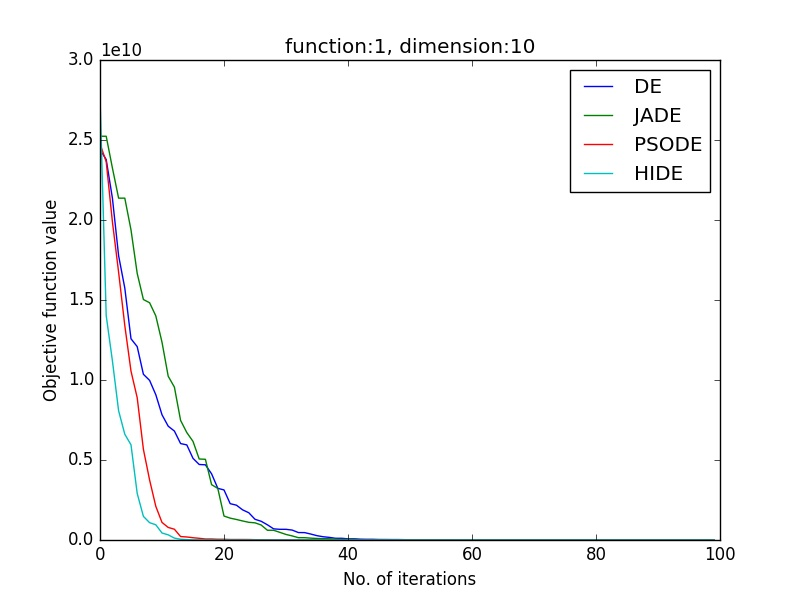
\includegraphics[width=\textwidth,natwidth=800,natheight=600]{F1D10}
        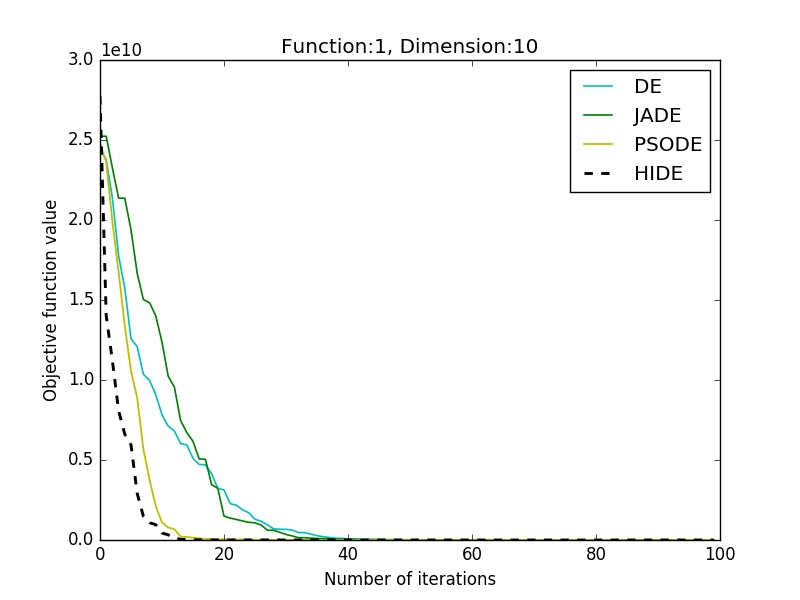
\includegraphics[width=\textwidth,natwidth=800,natheight=600]{plot_10D_F1_save}
        \caption{}
    \end{subfigure}
    \begin{subfigure}[b]{0.24\textwidth}
        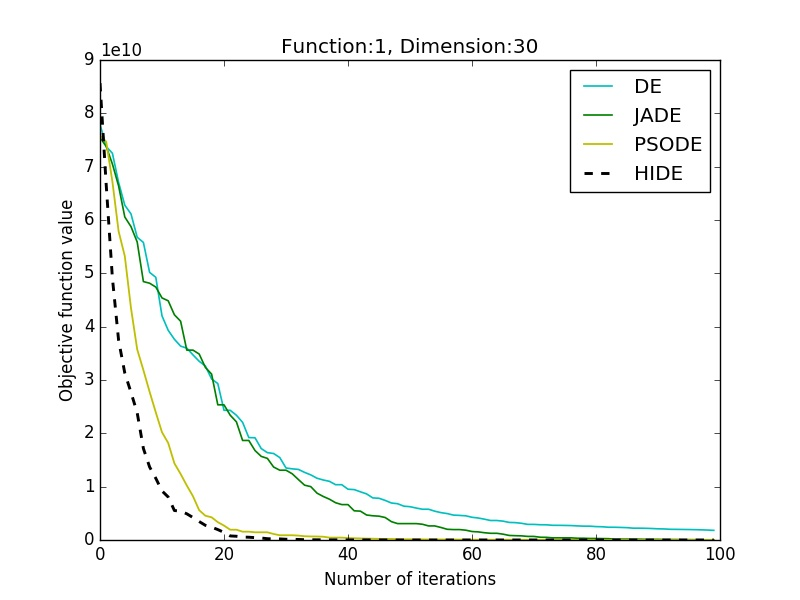
\includegraphics[width=\textwidth,natwidth=800,natheight=600]{plot_30D_F1_save}
        \caption{}
    \end{subfigure}    
    \begin{subfigure}[b]{0.24\textwidth}
        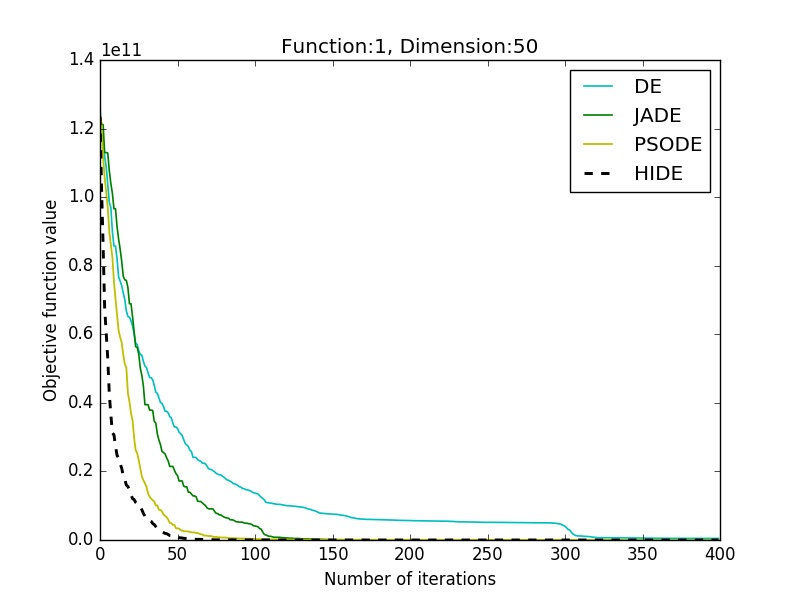
\includegraphics[width=\textwidth,natwidth=800,natheight=600]{plot_50D_F1_save}
        \caption{}
    \end{subfigure}
    \begin{subfigure}[b]{0.24\textwidth}
        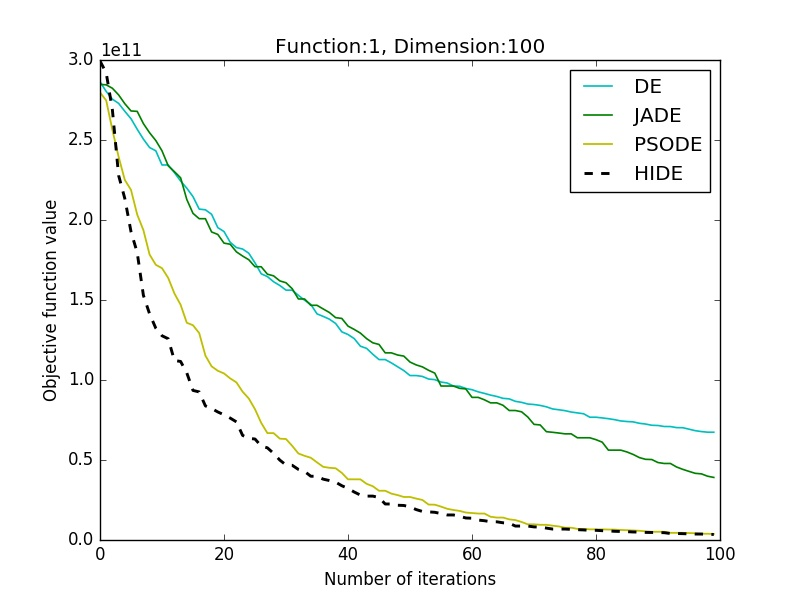
\includegraphics[width=\textwidth,natwidth=800,natheight=600]{plot_100D_F1_save}
        \caption{}
    \end{subfigure}

    \begin{subfigure}[b]{0.24\textwidth}
        % 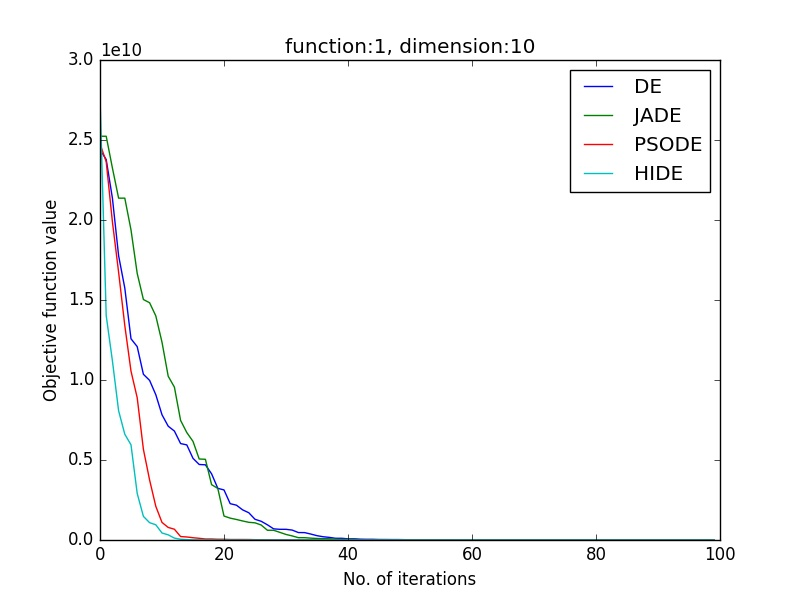
\includegraphics[width=\textwidth,natwidth=800,natheight=600]{F1D10}
        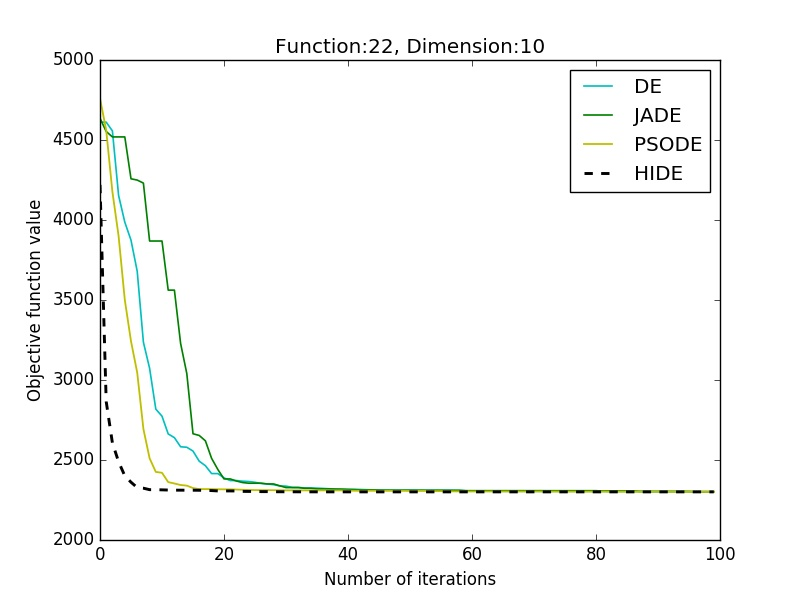
\includegraphics[width=\textwidth,natwidth=800,natheight=600]{plot_10D_F22_save}
        \caption{}
    \end{subfigure}
    \begin{subfigure}[b]{0.24\textwidth}
        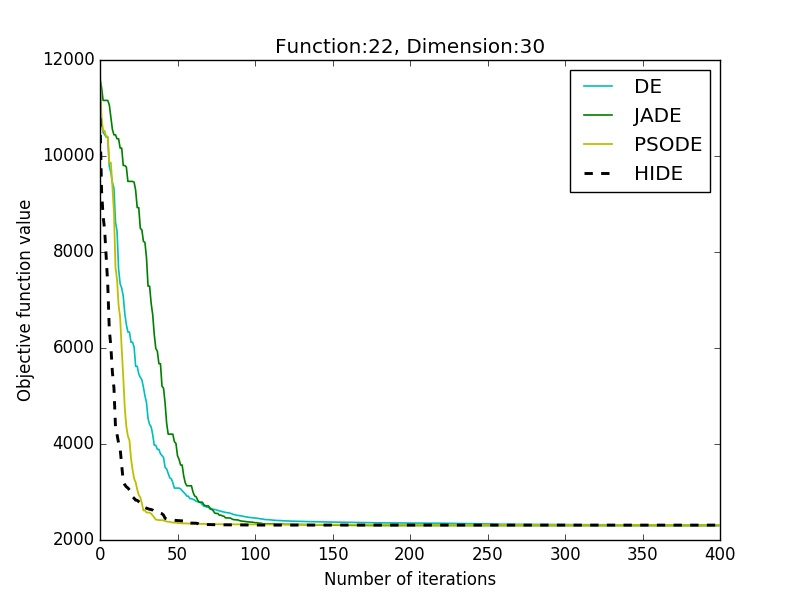
\includegraphics[width=\textwidth,natwidth=800,natheight=600]{plot_30D_F22_save}
        \caption{}
    \end{subfigure}    
    \begin{subfigure}[b]{0.24\textwidth}
        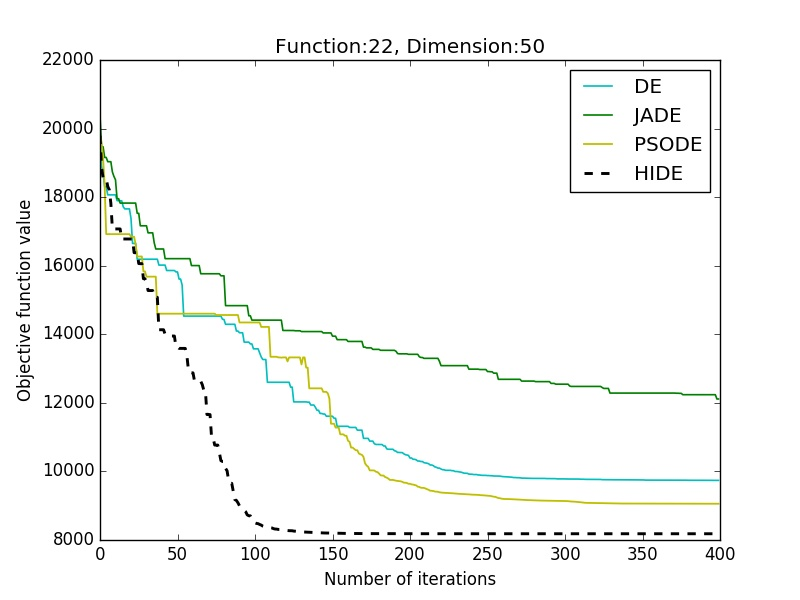
\includegraphics[width=\textwidth,natwidth=800,natheight=600]{plot_50D_F22_save}
        \caption{}
    \end{subfigure}
    \begin{subfigure}[b]{0.24\textwidth}
        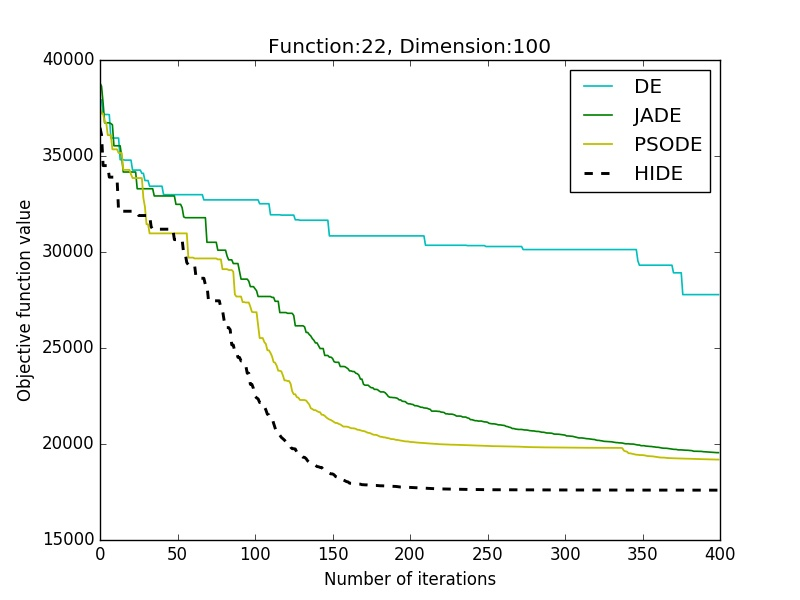
\includegraphics[width=\textwidth,natwidth=800,natheight=600]{plot_100D_F22_save}
        \caption{}
    \end{subfigure}

    \begin{subfigure}[b]{0.24\textwidth}
        % 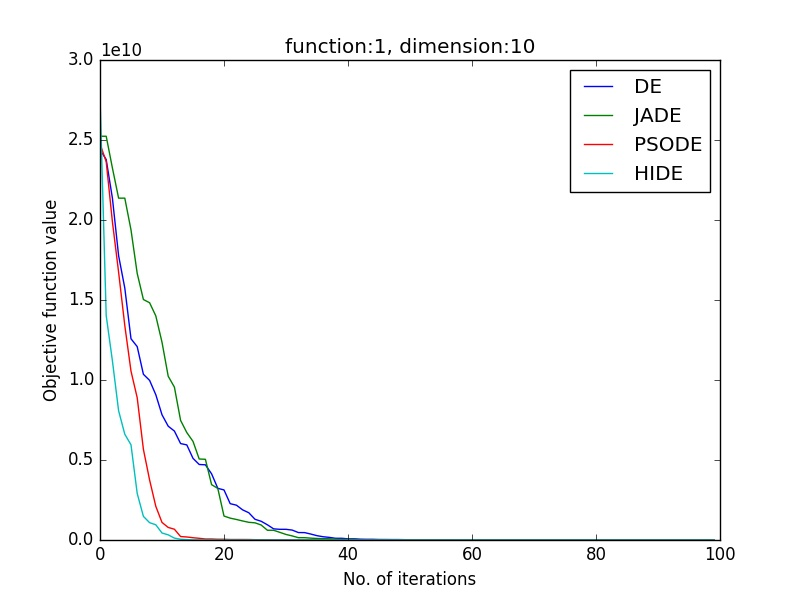
\includegraphics[width=\textwidth,natwidth=800,natheight=600]{F1D10}
        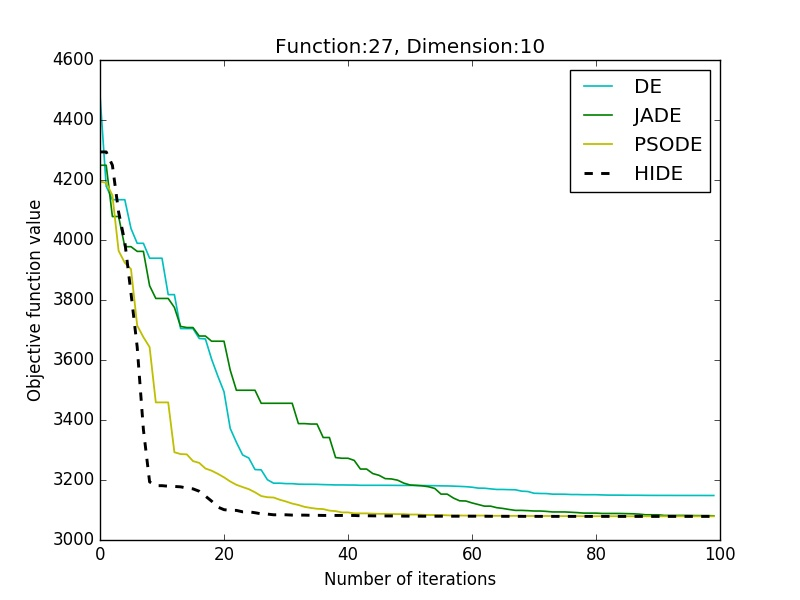
\includegraphics[width=\textwidth,natwidth=800,natheight=600]{plot_10D_F27_save}
        \caption{}
    \end{subfigure}
    \begin{subfigure}[b]{0.24\textwidth}
        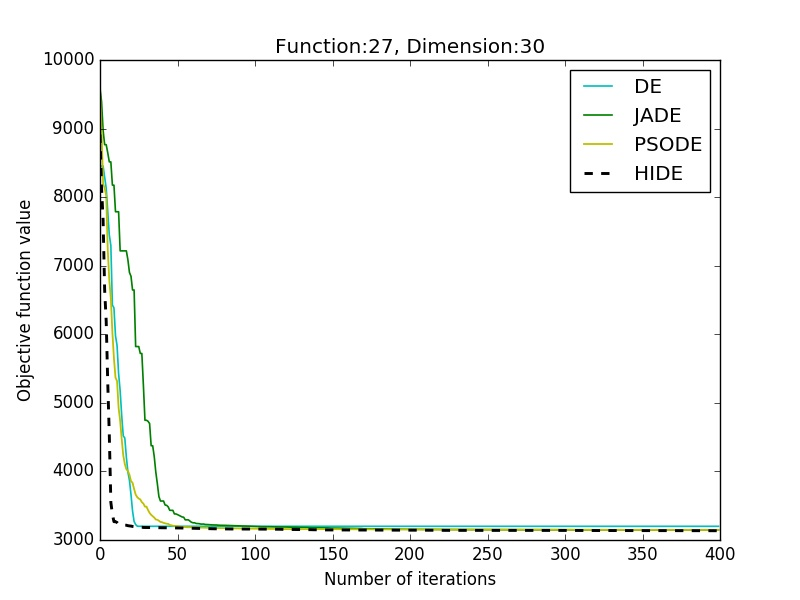
\includegraphics[width=\textwidth,natwidth=800,natheight=600]{plot_30D_F27_save}
        \caption{}
    \end{subfigure}    
    \begin{subfigure}[b]{0.24\textwidth}
        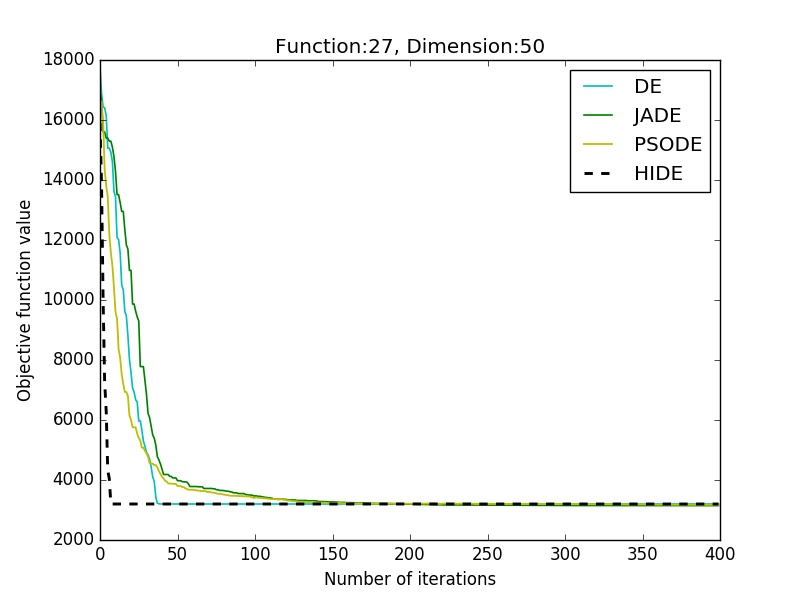
\includegraphics[width=\textwidth,natwidth=800,natheight=600]{plot_50D_F27_save}
        \caption{}
    \end{subfigure}
    \begin{subfigure}[b]{0.24\textwidth}
        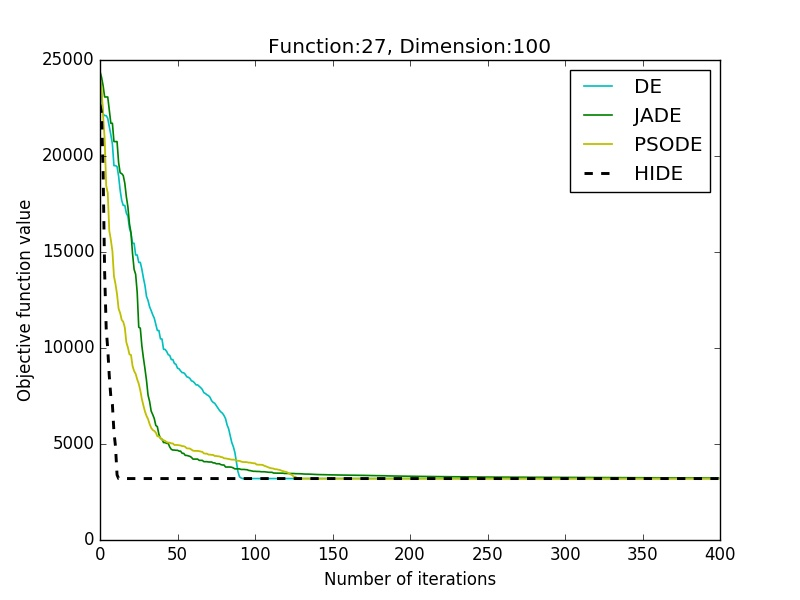
\includegraphics[width=\textwidth,natwidth=800,natheight=600]{plot_100D_F27_save}
        \caption{}
    \end{subfigure}

    \begin{subfigure}[b]{0.24\textwidth}
        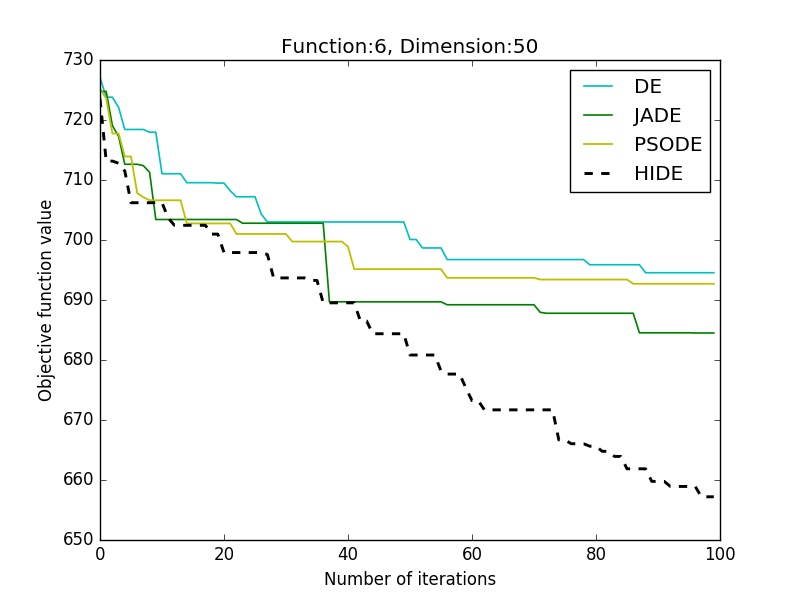
\includegraphics[width=\textwidth,natwidth=800,natheight=600]{plot_50D_F6_save}
        \caption{}
    \end{subfigure}
    \begin{subfigure}[b]{0.24\textwidth}
        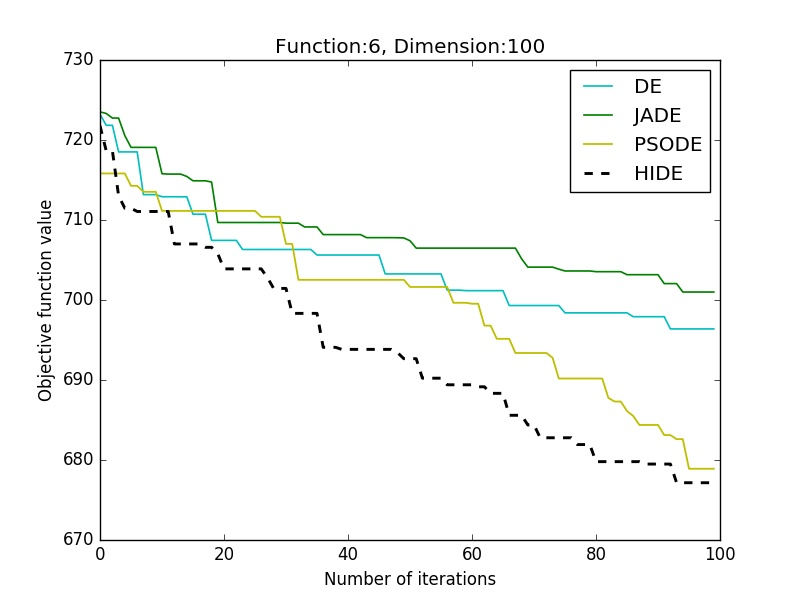
\includegraphics[width=\textwidth,natwidth=800,natheight=600]{plot_100D_F6_save}
        \caption{}
    \end{subfigure}        
    \begin{subfigure}[b]{0.24\textwidth}
        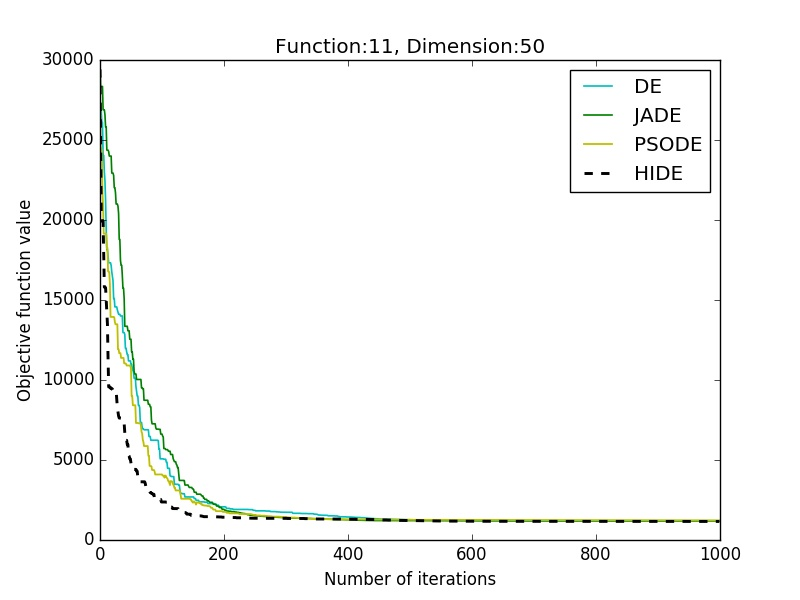
\includegraphics[width=\textwidth,natwidth=800,natheight=600]{plot_50D_F11_save}
        \caption{}
    \end{subfigure}
    \begin{subfigure}[b]{0.24\textwidth}
        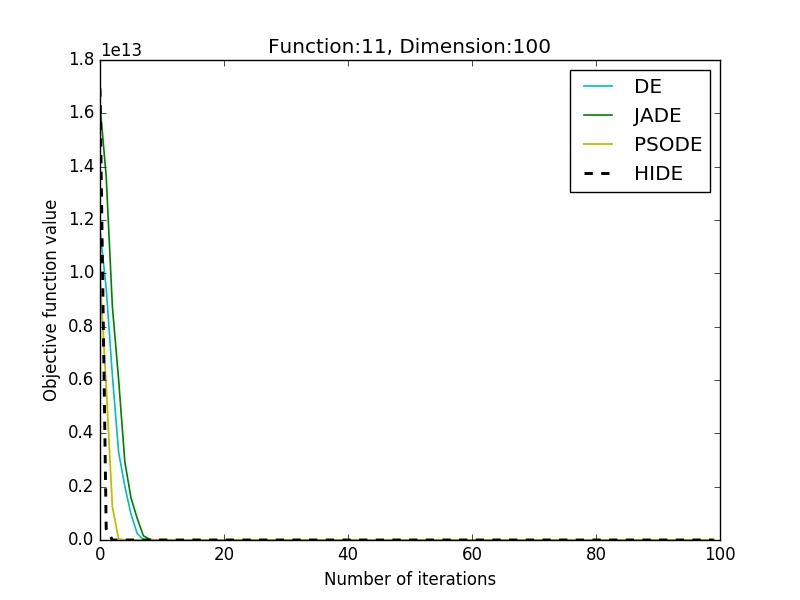
\includegraphics[width=\textwidth,natwidth=800,natheight=600]{plot_100D_F11_save}
        \caption{}
    \end{subfigure}

    \begin{subfigure}[b]{0.24\textwidth}
        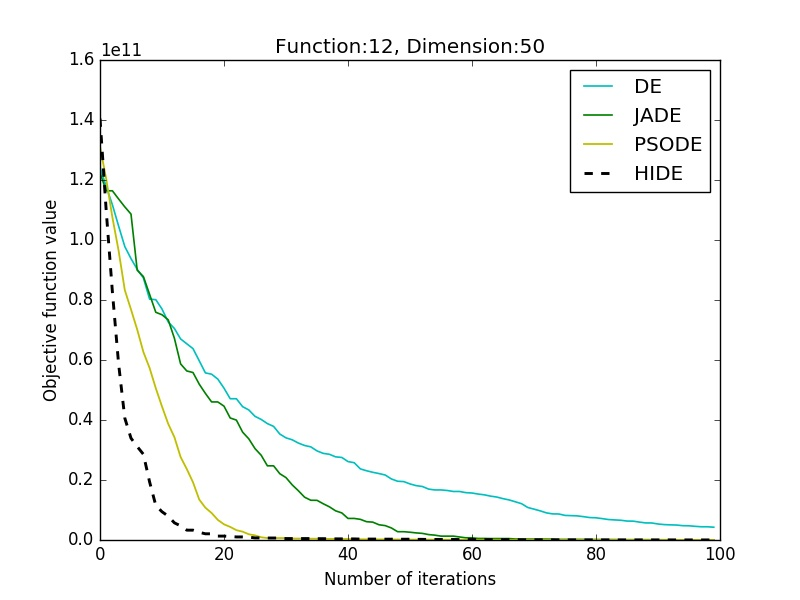
\includegraphics[width=\textwidth,natwidth=800,natheight=600]{plot_50D_F12_save}
        \caption{}
    \end{subfigure}
    \begin{subfigure}[b]{0.24\textwidth}
        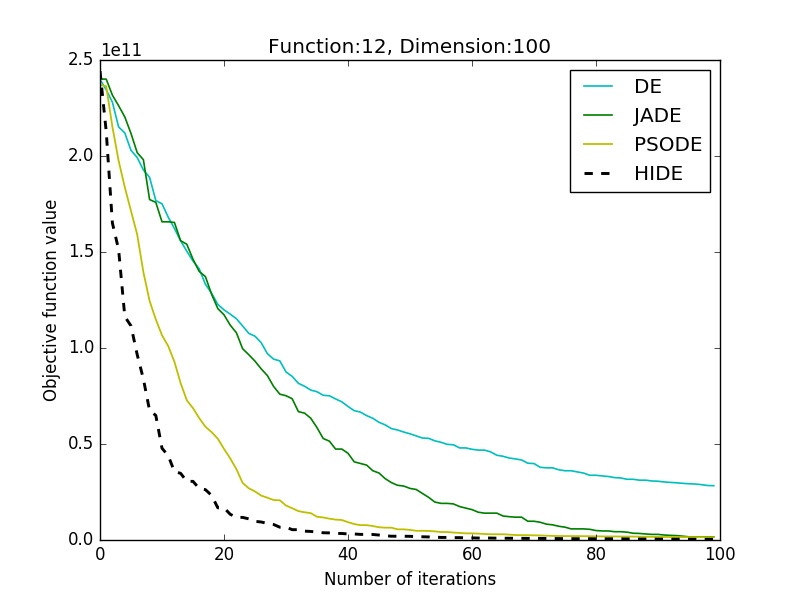
\includegraphics[width=\textwidth,natwidth=800,natheight=600]{plot_100D_F12_save}
        \caption{}
    \end{subfigure}
    \begin{subfigure}[b]{0.24\textwidth}
        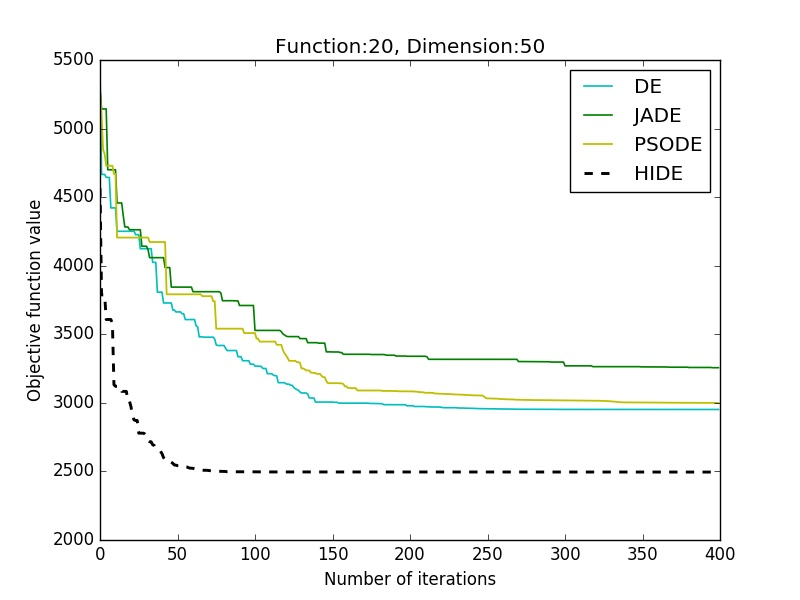
\includegraphics[width=\textwidth,natwidth=800,natheight=600]{plot_50D_F20_save}
        \caption{}
    \end{subfigure}
    \begin{subfigure}[b]{0.24\textwidth}
        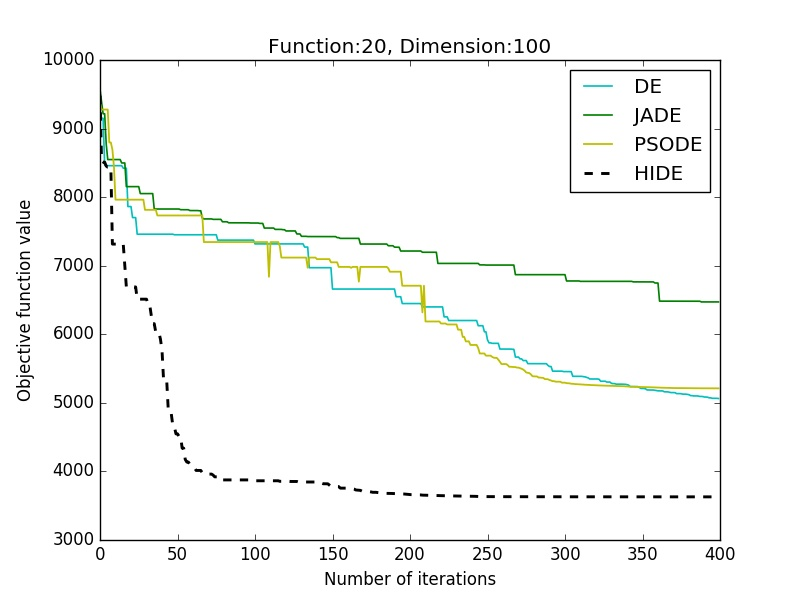
\includegraphics[width=\textwidth,natwidth=800,natheight=600]{plot_100D_F20_save}
        \caption{}
    \end{subfigure}

    \caption{Comparative convergence profiles for test functions from CEC 2017 Benchmark over D = 10,30,50,100}
    \vspace{-4mm}
\end{figure*}


\subsection{Numerical and Graphical Results} 
In tables 3-6, the best and mean values obtained for the population agents in the simulation runs have been reported, and the optimum values for each objective function have been highlighted in \textbf{bold}. For the sake of clarity, the comparison results in each table have been summarized in $"w/t/l"$ format wherein w represents the number of objective functions where the algorithm outperforms all other algorithms, t specifies the number of objective functions where it is tied as the best algorithm for the objective function and l represents the number of test functions where it does not finish first. The utilization of the evaluation metric facilitates a definitive comparison of the different algorithms under consideration.
 
Tables 3 and 4 highlight the performance of the algorithms for $D = 10$ and $D = 30$ respectively. For $D = 10$, HIDE depicits impressive performance. It registered a "$w/t/l$" score of $12/7/11$ in the best case and $14/4/12$ in the mean of population case. In both these test functions, JADE achieved the second best performance registering a w/t/l of $5/7/18$ on the best optimal value case and $9/4/17$ on the mean of optimal value case. On $D = 30$, HIDE achieved maximum number of wins in both best and mean case (17 and 18 respectively). JADE achieved second position with 8 and 9 wins in the best and mean case. The decent performance of JADE can be attributed to the adaptive nature of its parameter selection which enables enhancement of its convergence rate.

The results for $D = 50$ and $D = 100$ (higher dimensions) have been summarized in tables 5 and 6. On $D = 50$, HIDE depicted exceptional performance, outperforming all other algorithms. It registered 17 wins in the best case and 18 wins in the mean case. Classical DE shows no wins in any case in high dimensional settings owing to its slow convergence rate and inability to attain global optimum thus highlighting the usefulness of the modifications introduced in the variants including HIDE. Similarly for $D = 100$, HIDE again outperforms all other algorithms by an appreciable margin.
From a functional standpoint, It would be worthwhile to highlight that HIDE outperformed the other 3 compared algorithms on majority on the composite and hybrid functions, particularly on the higher dimensional settings. The efficiency of HIDE can be attributed to the hierarchical nature of crossover selection and concurrency in vector configurations at the higher hierarchy levels.
The tabular results reinforce the fact that HIDE outperforms JADE, PSODE and DE. On close analysis, it can be witnessed that HIDE falls behind the other algorithms on a small fraction of unimodal functions such as $f_5, f_7$ on lower dimensions due to fast convergence during early stages of execution. However, the performance of higher dimensions, particularly on the more involved functions highlights utility for real world problems.

The tabular results are complemented through the graphical representations in Figure 4. For the sake of clarity, representations of higher dimensional problems span more number of iterations than those for lower dimensional settings. Analysis of the plots clearly depicts that HIDE shows better convergence rate as compared to other algorithms. As the analysis transcends to higher dimensional settings, the proposed approach outperforms the other algorithms on majority of the objective functions with respect to both convergence rate and optimality. the superiority of our algorithm in higher dimensions (50 and 100) is clearly evident from Figure 4. (m,n,q,r,s,t). Figure 4. (e,f,g,h) depict that for functions where HIDE and the other variants may depict similar trends on lower dimensions, HIDE eventually excels and surpasses them in higher dimensions in most scenarios. Almost all figures are representative of a faster convergence rate for HIDE on higher dimensions. This remarkable trait in HIDE enhances its utility for high dimensional problems where fast convergence to global optimum value is required, hence making it superior to the other considered algorithms and several variants of the DE algorithm.


\section{Conclusion}

Differential Evolution has been regarded as one of the most successful optimization algorithms
and over the years, several variants have been proposed to enhance its convergence rate and performance. In the present work, we introduced a hierarchy influenced variant of the classical DE algorithm and modeled the same on the brain motor operation. The algorithm was characterized by global leader, local leaders and an effector population. The global leader and distributed local leaders interacted to facilitate gross motion via a greedy exploration strategy. The local leaders and their effectors interacted to control intricate motion for smooth convergence. A hierarchical crossover parameter was introduced to characterize the hierarchical transition between the two interactions. The influence of the vector configurations at the higher levels of hierarchy enabled the algorithm to avoid local minima in most objective functions. The same is complemented through our result observations wherein we significantly outperform several popular algorithm on complex multimodal functions in higher dimensional settings.
Our proposed approach has sought to establish a viable tradeoff between fast optimization, robust convergence and low number of control parameters.
The performance analysis of the algorithm highlights the particular effectiveness of the proposed approach on high dimensional hybrid and composite functions. The observed results provide sufficient motivation to extend the scope of the work to complex high dimensional real life problems including image enhancement, traveling salesman problem and flexible job-shop scheduling.


% \begin{acks}
%   The authors would like to thank Dr. Yuhua Li for providing the
%   matlab code of  the \textit{BEPS} method. 

%   The authors would also like to thank the anonymous referees for
%   their valuable comments and helpful suggestions. The work is
%   supported by the \grantsponsor{GS501100001809}{National Natural
%     Science Foundation of
%     China}{http://dx.doi.org/10.13039/501100001809} under Grant
%   No.:~\grantnum{GS501100001809}{61273304}
%   and~\grantnum[http://www.nnsf.cn/youngscientsts]{GS501100001809}{Young
%     Scientists' Support Program}.

% \end{acks}

% \subsection{Citations}
% Citations to articles~\cite{bowman:reasoning,
% clark:pct, braams:babel, herlihy:methodology},
% conference proceedings~\cite{clark:pct} or maybe
% books \cite{Lamport:LaTeX, salas:calculus} listed
% in the Bibliography section of your
% article will occur throughout the text of your article.
% You should use BibTeX to automatically produce this bibliography;
% you simply need to insert one of several citation commands with
% a key of the item cited in the proper location in
% the \texttt{.tex} file~\cite{Lamport:LaTeX}.
% The key is a short reference you invent to uniquely
% identify each work; in this sample document, the key is
% the first author's surname and a
% word from the title.  This identifying key is included
% with each item in the \texttt{.bib} file for your article.

% The details of the construction of the \texttt{.bib} file
% are beyond the scope of this sample document, but more
% information can be found in the \textit{Author's Guide},
% and exhaustive details in the \textit{\LaTeX\ User's
% Guide}~\cite{Lamport:LaTeX}.

% This article shows only the plainest form
% of the citation command, using \texttt{{\char'134}cite}.


% \subsection{Type Changes and {\itshape Special} Characters}

% We have already seen several typeface changes in this sample.  You can
% indicate italicized words or phrases in your text with the command
% \texttt{{\char'134}textit}; emboldening with the command
% \texttt{{\char'134}textbf} and typewriter-style (for instance, for
% computer code) with \texttt{{\char'134}texttt}.  But remember, you do
% not have to indicate typestyle changes when such changes are part of
% the \textit{structural} elements of your article; for instance, the
% heading of this subsection will be in a sans serif\footnote{Another
%   footnote, here.  Let's make this a rather short one to see how it
%   looks.} typeface, but that is handled by the document class file.
% Take care with the use of\footnote{A third, and last, footnote.}  the
% curly braces in typeface changes; they mark the beginning and end of
% the text that is to be in the different typeface.

% You can use whatever symbols, accented characters, or non-English
% characters you need anywhere in your document; you can find a complete
% list of what is available in the \textit{\LaTeX\ User's Guide}
% \cite{Lamport:LaTeX}.

% \subsection{Math Equations}
% You may want to display math equations in three distinct styles:
% inline, numbered or non-numbered display.  Each of
% the three are discussed in the next sections.

% \subsubsection{Inline (In-text) Equations}
% A formula that appears in the running text is called an
% inline or in-text formula.  It is produced by the
% \textbf{math} environment, which can be
% invoked with the usual \texttt{{\char'134}begin\,\ldots{\char'134}end}
% construction or with the short form \texttt{\$\,\ldots\$}. You
% can use any of the symbols and structures,
% from $\alpha$ to $\omega$, available in
% \LaTeX~\cite{Lamport:LaTeX}; this section will simply show a
% few examples of in-text equations in context. Notice how
% this equation:
% \begin{math}
%   \lim_{n\rightarrow \infty}x=0
% \end{math},
% set here in in-line math style, looks slightly different when
% set in display style.  (See next section).

% \subsubsection{Display Equations}
% A numbered display equation---one set off by vertical space from the
% text and centered horizontally---is produced by the \textbf{equation}
% environment. An unnumbered display equation is produced by the
% \textbf{displaymath} environment.

% Again, in either environment, you can use any of the symbols
% and structures available in \LaTeX\@; this section will just
% give a couple of examples of display equations in context.
% First, consider the equation, shown as an inline equation above:
% \begin{equation}
%   \lim_{n\rightarrow \infty}x=0
% \end{equation}
% Notice how it is formatted somewhat differently in
% the \textbf{displaymath}
% environment.  Now, we'll enter an unnumbered equation:
% \begin{displaymath}
%   \sum_{i=0}^{\infty} x + 1
% \end{displaymath}
% and follow it with another numbered equation:
% \begin{equation}
%   \sum_{i=0}^{\infty}x_i=\int_{0}^{\pi+2} f
% \end{equation}
% just to demonstrate \LaTeX's able handling of numbering.


% \subsection{Tables}
% Because tables cannot be split across pages, the best
% placement for them is typically the top of the page
% nearest their initial cite.  To
% ensure this proper ``floating'' placement of tables, use the
% environment \textbf{table} to enclose the table's contents and
% the table caption.  The contents of the table itself must go
% in the \textbf{tabular} environment, to
% be aligned properly in rows and columns, with the desired
% horizontal and vertical rules.  Again, detailed instructions
% on \textbf{tabular} material
% are found in the \textit{\LaTeX\ User's Guide}.

% Immediately following this sentence is the point at which
% Table~\ref{tab:freq} is included in the input file; compare the
% placement of the table here with the table in the printed
% output of this document.

% \begin{table}
%   \caption{Frequency of Special Characters}
%   \label{tab:freq}
%   \begin{tabular}{ccl}
%     \toprule
%     Non-English or Math&Frequency&Comments\\
%     \midrule
%     \O & 1 in 1,000& For Swedish names\\
%     $\pi$ & 1 in 5& Common in math\\
%     \$ & 4 in 5 & Used in business\\
%     $\Psi^2_1$ & 1 in 40,000& Unexplained usage\\
%   \bottomrule
% \end{tabular}
% \end{table}

% To set a wider table, which takes up the whole width of the page's
% live area, use the environment \textbf{table*} to enclose the table's
% contents and the table caption.  As with a single-column table, this
% wide table will ``float'' to a location deemed more desirable.
% Immediately following this sentence is the point at which
% Table~\ref{tab:commands} is included in the input file; again, it is
% instructive to compare the placement of the table here with the table
% in the printed output of this document.


% \begin{table*}
%   \caption{Some Typical Commands}
%   \label{tab:commands}
%   \begin{tabular}{ccl}
%     \toprule
%     Command &A Number & Comments\\
%     \midrule
%     \texttt{{\char'134}author} & 100& Author \\
%     \texttt{{\char'134}table}& 300 & For tables\\
%     \texttt{{\char'134}table*}& 400& For wider tables\\
%     \bottomrule
%   \end{tabular}
% \end{table*}
% % end the environment with {table*}, NOTE not {table}!

% It is strongly recommended to use the package booktabs~\cite{Fear05}
% and follow its main principles of typography with respect to tables:
% \begin{enumerate}
% \item Never, ever use vertical rules.
% \item Never use double rules.
% \end{enumerate}
% It is also a good idea not to overuse horizontal rules.


% \subsection{Figures}

% Like tables, figures cannot be split across pages; the best placement
% for them is typically the top or the bottom of the page nearest their
% initial cite.  To ensure this proper ``floating'' placement of
% figures, use the environment \textbf{figure} to enclose the figure and
% its caption.

% This sample document contains examples of \texttt{.eps} files to be
% displayable with \LaTeX.  If you work with pdf\LaTeX, use files in the
% \texttt{.pdf} format.  Note that most modern \TeX\ systems will convert
% \texttt{.eps} to \texttt{.pdf} for you on the fly.  More details on
% each of these are found in the \textit{Author's Guide}.

% \begin{figure}
% 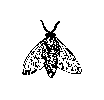
\includegraphics{fly}
% \caption{A sample black and white graphic.}
% \end{figure}

% \begin{figure}
% 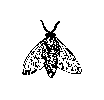
\includegraphics[height=1in, width=1in]{fly}
% \caption{A sample black and white graphic
% that has been resized with the \texttt{includegraphics} command.}
% \end{figure}


% As was the case with tables, you may want a figure that spans two
% columns.  To do this, and still to ensure proper ``floating''
% placement of tables, use the environment \textbf{figure*} to enclose
% the figure and its caption.  And don't forget to end the environment
% with \textbf{figure*}, not \textbf{figure}!

% \begin{figure*}
% 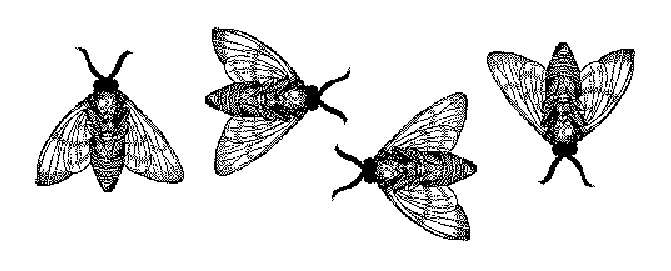
\includegraphics{flies}
% \caption{A sample black and white graphic
% that needs to span two columns of text.}
% \end{figure*}


% \begin{figure}
% 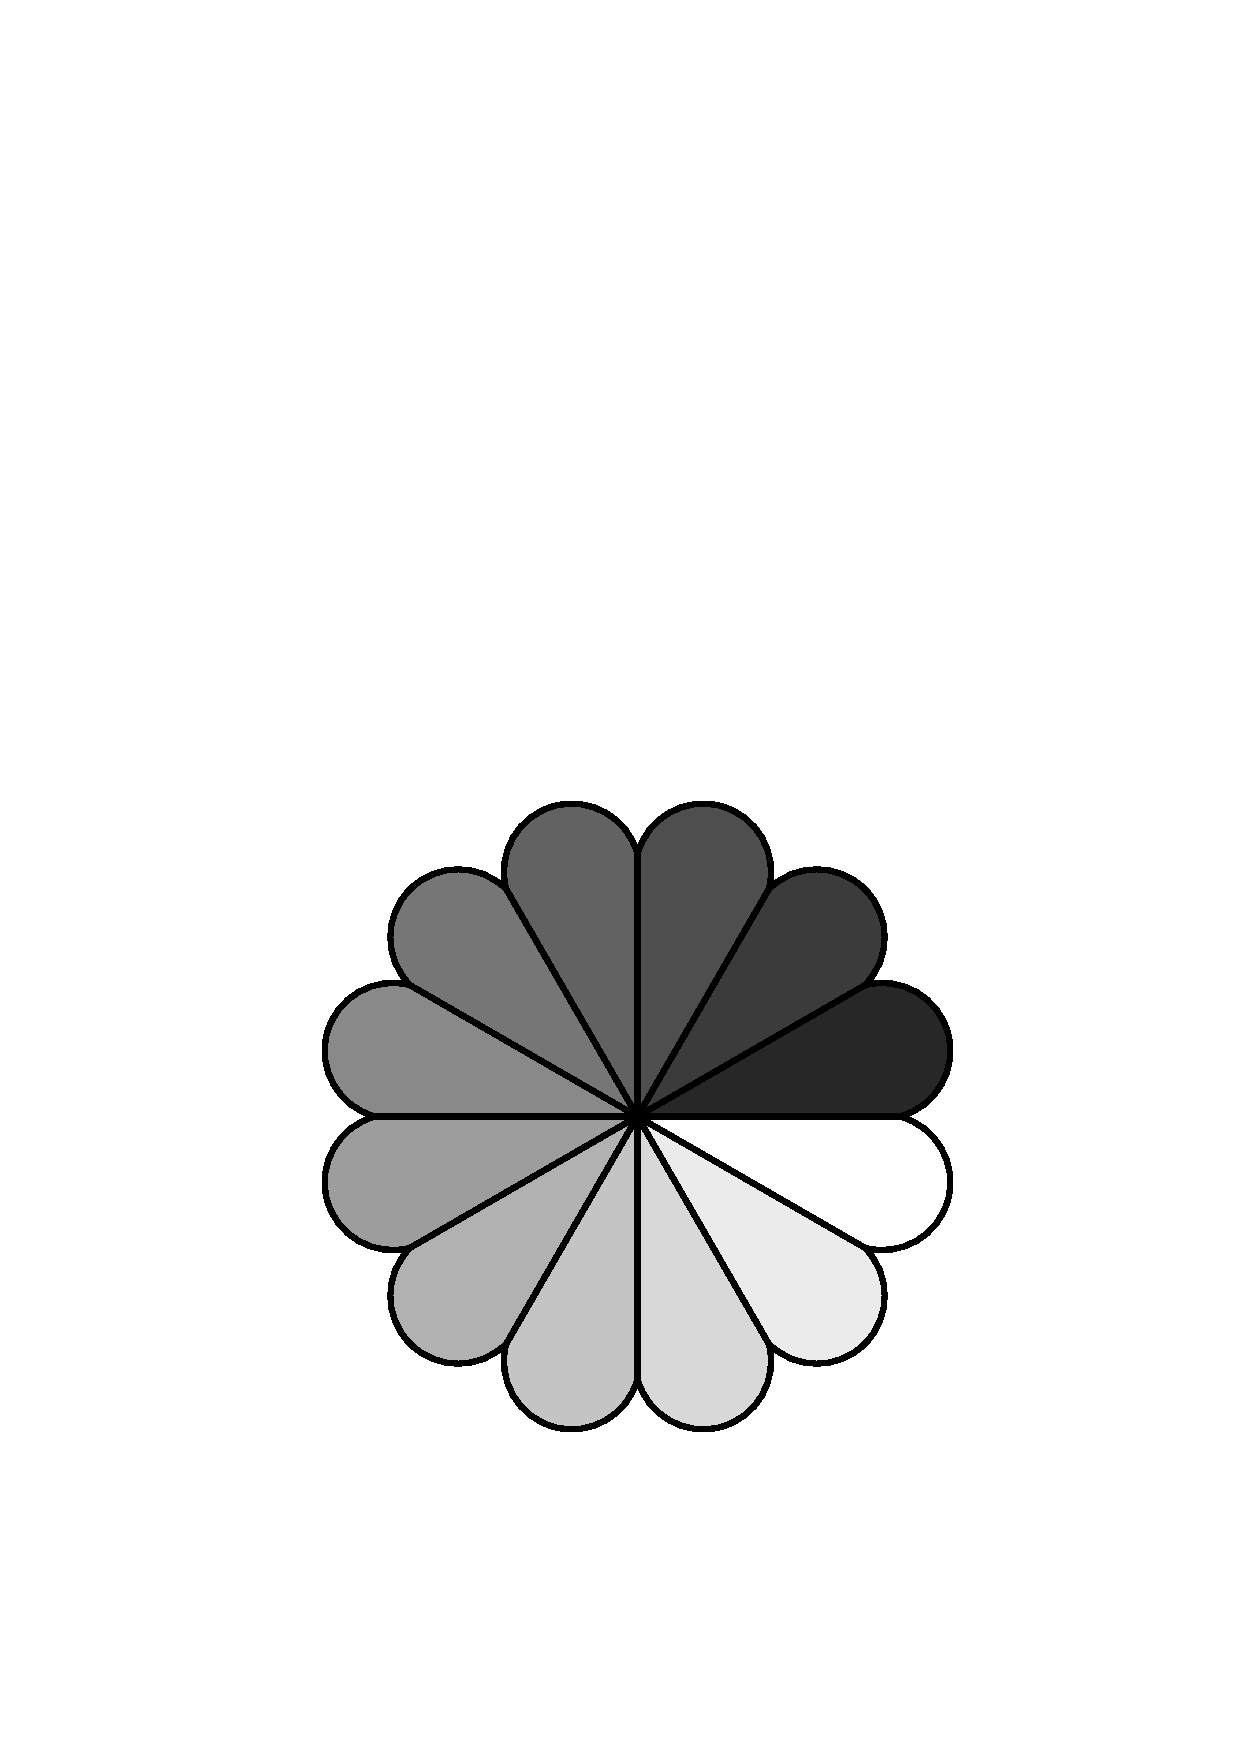
\includegraphics[height=1in, width=1in]{rosette}
% \caption{A sample black and white graphic that has
% been resized with the \texttt{includegraphics} command.}
% \end{figure}

% \subsection{Theorem-like Constructs}

% Other common constructs that may occur in your article are the forms
% for logical constructs like theorems, axioms, corollaries and proofs.
% ACM uses two types of these constructs:  theorem-like and
% definition-like.

% Here is a theorem:
% \begin{theorem}
%   Let $f$ be continuous on $[a,b]$.  If $G$ is
%   an antiderivative for $f$ on $[a,b]$, then
%   \begin{displaymath}
%     \int^b_af(t)\,dt = G(b) - G(a).
%   \end{displaymath}
% \end{theorem}

% Here is a definition:
% \begin{definition}
%   If $z$ is irrational, then by $e^z$ we mean the
%   unique number that has
%   logarithm $z$:
%   \begin{displaymath}
%     \log e^z = z.
%   \end{displaymath}
% \end{definition}

% The pre-defined theorem-like constructs are \textbf{theorem},
% \textbf{conjecture}, \textbf{proposition}, \textbf{lemma} and
% \textbf{corollary}.  The pre-defined de\-fi\-ni\-ti\-on-like constructs are
% \textbf{example} and \textbf{definition}.  You can add your own
% constructs using the \textsl{amsthm} interface~\cite{Amsthm15}.  The
% styles used in the \verb|\theoremstyle| command are \textbf{acmplain}
% and \textbf{acmdefinition}.

% Another construct is \textbf{proof}, for example,

% \begin{proof}
%   Suppose on the contrary there exists a real number $L$ such that
%   \begin{displaymath}
%     \lim_{x\rightarrow\infty} \frac{f(x)}{g(x)} = L.
%   \end{displaymath}
%   Then
%   \begin{displaymath}
%     l=\lim_{x\rightarrow c} f(x)
%     = \lim_{x\rightarrow c}
%     \left[ g{x} \cdot \frac{f(x)}{g(x)} \right ]
%     = \lim_{x\rightarrow c} g(x) \cdot \lim_{x\rightarrow c}
%     \frac{f(x)}{g(x)} = 0\cdot L = 0,
%   \end{displaymath}
%   which contradicts our assumption that $l\neq 0$.
% \end{proof}

% \section{Conclusions}
% This paragraph will end the body of this sample document.
% Remember that you might still have Acknowledgments or
% Appendices; brief samples of these
% follow.  There is still the Bibliography to deal with; and
% we will make a disclaimer about that here: with the exception
% of the reference to the \LaTeX\ book, the citations in
% this paper are to articles which have nothing to
% do with the present subject and are used as
% examples only.
% %\end{document}  % This is where a 'short' article might terminate



% \appendix
% %Appendix A
% \section{Headings in Appendices}
% The rules about hierarchical headings discussed above for
% the body of the article are different in the appendices.
% In the \textbf{appendix} environment, the command
% \textbf{section} is used to
% indicate the start of each Appendix, with alphabetic order
% designation (i.e., the first is A, the second B, etc.) and
% a title (if you include one).  So, if you need
% hierarchical structure
% \textit{within} an Appendix, start with \textbf{subsection} as the
% highest level. Here is an outline of the body of this
% document in Appendix-appropriate form:
% \subsection{Introduction}
% \subsection{The Body of the Paper}
% \subsubsection{Type Changes and  Special Characters}
% \subsubsection{Math Equations}
% \paragraph{Inline (In-text) Equations}
% \paragraph{Display Equations}
% \subsubsection{Citations}
% \subsubsection{Tables}
% \subsubsection{Figures}
% \subsubsection{Theorem-like Constructs}
% \subsubsection*{A Caveat for the \TeX\ Expert}
% \subsection{Conclusions}
% \subsection{References}
% Generated by bibtex from your \texttt{.bib} file.  Run latex,
% then bibtex, then latex twice (to resolve references)
% to create the \texttt{.bbl} file.  Insert that \texttt{.bbl}
% file into the \texttt{.tex} source file and comment out
% the command \texttt{{\char'134}thebibliography}.
% % This next section command marks the start of
% % Appendix B, and does not continue the present hierarchy
% \section{More Help for the Hardy}

% Of course, reading the source code is always useful.  The file
% \path{acmart.pdf} contains both the user guide and the commented
% code.


